\chapter{基于深度学习的天波超视距雷达地海杂波识别}
\section{引言}

\textcolor{red}{该章可以添加利用二维卷积神经网络进行识别的算法实验}
\textcolor{red}{复合类的提取}

\textcolor{red}{该部分仍然存在问题}

天波超视距雷达利用电磁波在电离层与地/海面之间的反射作用传输高频能量,其作用距离不受地球曲率的限制,可实现对隐身战斗机、洲际导弹、巡航导弹、大中型舰船等高价值目标的远程预警,受到世界各国的高度关注。天波超视距雷达系统主要由主雷达和电离层探测子系统组成,其中后者为前者提供电离层传播条件评估以及坐标配准参数等。由于电离层探测子系统独立于主雷达工作,因此其提供的坐标配准参数与主雷达量测回波存在不一致性、误差大等问题,从而造成电离层传播模式识别正确率低、目标定位精度差等。一种改进方式是通过设置有源信标提供坐标配准修正参数,但是受到可部署区域的限制。由于陆地、海洋对雷达信号散射特性不同,可将陆地、海洋地理信息作为一类无源信标。通过区分识别地海杂波、构建地海边界轮廓、与先验地理轮廓信息匹配可同样提供坐标配准修正参数。传统地海杂波识别算法难以准确提取及表达地海杂波特征,从而在复杂电离层状况下地海杂波识别正确率较低。因此,如何发展一种更加准确的地海杂波类型识别方法,对天波超视距雷达电离层参数辨识及目标定位精度的提升有着重要意义。

本章解决了在复杂的电离层环境下天波超视距雷达地海杂波类型的识别问题。本章构建了适用于天波超视距雷达地海杂波类型识别的卷积神经网络,利用大量训练数据对卷积神经网络进行训练,提取合理的特征;然后,利用提取的特征对实时雷达地海杂波回波进行在线分类识别。本章要解决的技术问题是提供一种新的基于深度神经网络的地海杂波识别技术,避免了手工提取地海杂波特征。本章所提出的算法大大提高了天波超视距雷达地海杂波的识别正确率与实时性。

天波超视距雷达由于受雷达工作机制及其电波环境的影响,特别是受电离层多模多路径影响,目标回波-传播模式正确配对很困难,目标检测和定位精度较低。为了提升目标定位经度,一种设想是利用检测区域内的有源/无源信标进行目标位置修正处理,通过对地海杂波特征深入分析和研究,分类识别出地海杂波,提取地海特征信息,并通过与地理位置匹配处理产生修正参数等,从而解决电离层模式配对等诸多工程应用问题,达到提升目标定位精度的目的。同时,在海杂波背景中探测海绵舰船目标的环境极其复杂,由于电波传播环境的影响(电离层时变和失真、易受干扰等),地海杂波附近存在很多虚警回波,严重影响目标的发现和自适应跟踪处理。为提升对舰船目标的处理能力,有必要研究新的处理方法,既能有效抑制虚警杂波,又能识别出感兴趣的低速舰船目标并稳定跟踪。

\begin{figure}[!t]
	\centering
	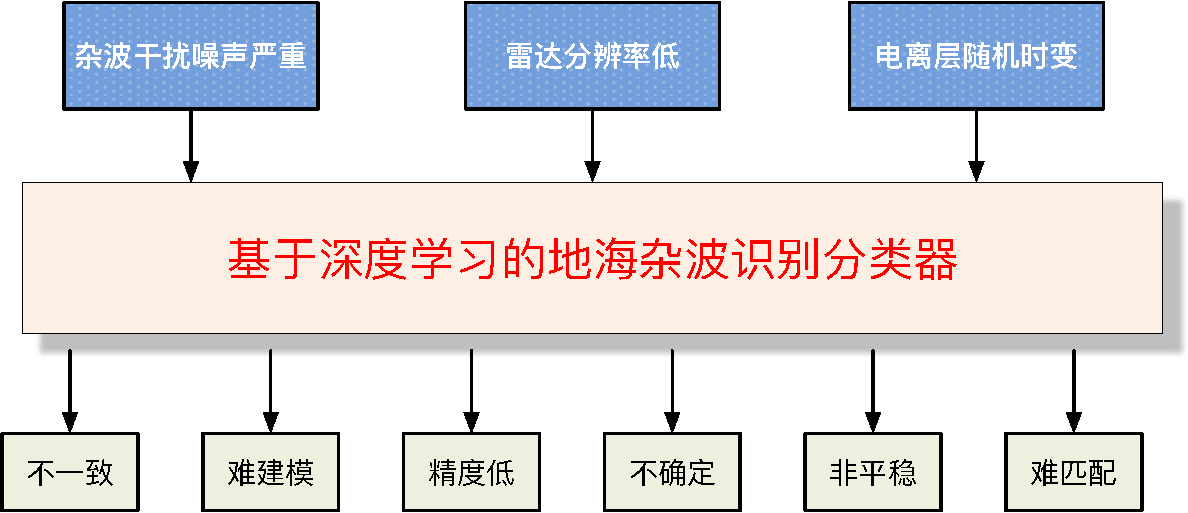
\includegraphics[width=\textwidth]{figures/clutterproblem.pdf}
	\caption{某距离方位单元海杂波频谱数据关注度图
	。}
	\label{fig:visfeature}
\end{figure}

天波超视距雷达目标定位精度依赖于传播模式的准确识别以及PD变换系数的精确测量。电离层传播的复杂性使得传播模式很难精确确定,而电离层探测子系统独立于主雷达工作导致其提供的坐标配准参数与主雷达量测回波存在不一致性、误差大等问题,从而造成电离层传播模式识别正确率低、目标定位精度差等。天波超视距雷达地海杂波识别是一种基于无源信标(远海区域的岛屿等陆地)获得PD变换系数的技术。鉴于远海地区有源设备的布置面临着较大的困难,通过区分识别地海杂波、构建地海边界轮廓、与先验地理轮廓信息匹配可同样提供坐标配准修正参数,改善周围航迹目标的定位精度。受分辨率低、定位精度差、系统偏差大、电离层多模、多路径传播等因素影响,天波雷达地海杂波识别技术存在很大挑战,主要体现在以下几个方面:
\begin{itemize}
	\item 天波雷达的距离分辨率为7.5-30公里,方位分辨率为0.582-1.067°,低分辨率影响地海特性的判别以及匹配精度;
	\item 离层状况变化情况十分复杂,导致地海杂波的特性并不稳定,区分地海杂波特性的布拉格峰会发生偏移甚至某个峰会消失,对地海杂波的建模影响很大;
	\item 确定修正系数对周围区域航迹的修正范围、有效性等难度大,需要大量实装数据验证;
\end{itemize}

因此,一些作者提出了一种使用岛屿作为无源信标的方法来寻找PD变换系数\cite{cuccoli2011coordinate}的方法。我们可以根据频谱数据识别出地海分界线,进而确定出岛屿在雷达坐标系中的位置,然后将其与地理坐标中的岛屿对应。因此,我们可以根据相同位置基准的偏差来获得PD变换系数。因此,这种方法最基础和最关键的部分是识别地海杂波识别。

上述所有作者的研究重点主要是如何通过地理坐标的匹配来进行求取变换系数,而对于地海杂波识别方面的研究却并不多。靳珍璐等\cite{jin2012svm}提出了一种基于支持向量机(Support Vector Machine,SVM)的识别算法。他们通过使用三种地海杂波频谱特征来训练SVM,并用仿真数据进行验证。然而,在实际情况下,地海杂波的特征取决于当时的电离层环境、雷达的扫掠角度、天气环境等,地海杂波模型有十分强的不确定性。当建模所需的参数变化时,算法的准确性将急剧下降。2013年,Li等\cite{li2013high} 使用神经网络方法解决了一个和我们问题十分相似的飞机检测问题。

\textcolor{red}{在本章中,我们采用深度学习方法,特别是深层卷积神经网络来解决天波超视距雷达的地海波识别。通过分析天波雷达收到的地海回波频谱数据的特征,我们发现...基于深度学习方法,符合分类器优势的资格。}

一种方法是利用建立基于先验信息的电离层统计模型,另一种方法是通过一些检测设备收集信息。但是这两种方法都有一些限制,前者无法及时更新,有时会产生严重错误(如天气突变情况),后者需要大量设备,并且不容易将其放置在远海地区。

我们利用不同电离层条件、雷达工作条件、位置和时间下的频谱数据来进行算法的验证。不同的时间和地理位置对应于不同的电离层条件,不同的电离层条件将严重影响频谱的状态。对于不同的雷达工作条件,由于发射频率变化,回波频谱密度和幅度也将随之变化。通过观察、学习大量不同条件的频谱数据,可以更全面地区分地海杂波。

\subsection{地海杂波识别分析}
天波超视距雷达目标的坐标配准问题在很大程度上影响了其跟踪精度,特别是对于电离层参数无法准确及时获得的较远。识别地海分界线主要有两个优点:第一个是我们可以使用获取的杂波地形图与实际的地图进行匹配,然后根据匹配结果计算偏移量,得到坐标修正系数,用来提高目标跟踪精度;另一方面,我们可以利用由识别结果获得的频谱上的偏移来校正频谱本身,以提高目标检测概率和准确度。

天波超视距雷达频谱数据的地海杂波识别有两个独特的挑战。第一个是难以对杂波进行建模,由于电离层模型变化较大导致杂波模型混乱且复杂性较高。传统的建模方法一般根据实际数据选取一种分布来描述雷达杂波,如瑞利分布(Rayleigh distribution),威布尔分布(Weibull distribution),K分布(K distribution)等。但天波超视距雷达获得的杂波模型一直变化,这种建模方法不能得到很好的结果。其次,传统的地海杂波的分类特征很难定量描述。一个熟练的操作人员可能很熟练地区分出地海杂波,但是这部分却很难利用数学模型对其描述。本章我们提出了一种新的可以有效解决上述挑战的利用深度卷积神经网络的方法。我们的算法将CNN应用于地海杂波识别。我们避免了对杂波进行建模选取特征的方法,从根本上避免了传统方法所面临的困难。

本节将我们提出的算法与传统工程中常用的单阈值法和支持向量机方法进行了对比,我们发现:
\begin{itemize}
	\item 我们基于卷积神经网络的方法中获得最好的结果,且在地图匹配结果方面显著优于其余两种方法。
	\item 我们的方法具有很强的鲁棒性,雷达参数或者自然变化对识别结果影响不大。
\end{itemize}
我们初步对我们基于深度卷积神经网络的地海杂波分类算法进行了可行性分析,从结果可以看出其明显优于其余两种算法。另一方面,如果我们针对于特定的问题对卷积神经网络的参数进行调整,可以进一步提高我们算法的性能。
\subsection{我们的方法}
天波超视距雷达地海杂波识别技术的处理流程可分为信息预处理、地海杂波识别、地理位置匹配、定位精度提升四个处理层。 图 1系统结构图具体过程为:对频谱数据进行清洗、裁剪、融合等预处理操作,将预处理过的整体频谱数据输入到已经训练好的深度卷积神经网络分类器中进行识别,并将识别结果与二值化的地图模板进行匹配,从而得到匹配结果进而得到修正系数。最终将修正系数应用于目标跟踪过程,提升定位精度。

深度学习体系结构中有几大网络模型,其中的卷积神经网络可以直接将整个需要分类的数据作为网络的输入,避免了传统识别算法中复杂的特征提取和数据重建过程。基于此优点,使卷积神经网络在本章所需解决的天波超视距雷达地海杂波特征识别问题中有着巨大优势。

典型的卷积神经网络由深层结构堆叠在一起的多个不同的层组成:输入层,多组卷积和池化层,有限数量的完全连接的隐藏层,以及输出层。其中最主要的部分为卷积层。其利用输入数据中的局部结构,将整个输入空间划分成很小的隐藏单元。将各个隐藏单元的权重构建得到的卷积核作用于整个输入空间,从而得到特征向量。利用这种机制,我们不仅大大减少了参数数量同时提高了数据的平移不变性。

\textcolor{blue}{本章根据地海杂波频谱的实际数据以及其反映出来的特性,构建了基本的具有3 层隐藏层的深度卷积神经网络,每层具有多个特征向量,每个特征向量具有多个神经元,并且每个特征向量来自于一种卷积核所提取输入的一种特征。
}

频谱数据预处理频谱数据是从天波超视距雷达获取的多普勒频率与幅度值对应的数据。在利用数据之前,我们首先对该数据进行清洗,把下图这种并非处于正常探测模式下的数据进行去除。 图 3 需要被清洗掉的数据由于数据来自不同波位、不同时刻,具有不同的雷达工作频率,我们在利用这些数据进行训练或者识别前需要首先对其进行基本的处理。主要包括将数据按照积累点数、波位和多普勒频率范围进行分类,不同类别的数据分开处理。另一方面,由于地海杂波特征主要集中于多普勒频率较低的区域,我们可以将数据进行裁剪,只选取有效数据(本课题中在权衡信息保留以及计算量的清洗下,保留了处于零频附近,且频率范围为整体一半的区域),在一定程度上减小计算量。 图 4 数据裁剪示意图受电离层非平稳、时变等特性影响,天波超视距雷达杂波数据可能会出现较大波动。对这种波动不加处理会导致地海杂波识别结果不准确。在一个相对短时间内,电离层会保持一个较平稳的状态,也即同一距离、方位单元的真实的地海属性不会发生变化。因此,本课题在频谱数据预处理阶段采用滑窗融合的思想,将连续窗长时间 内的相邻杂波数据 进行加权融合得到新的频谱数据作为深度卷积神经网络分类器的输入 ,其中 为频谱数据 的权重,关于窗长及权重的选择会在后面技术方案验证部分进行详细的讨论。

卷积神经网络(Convolution neural network,CNN)是深度学习中的一种重要算法,在分类等领域具有很大的优势。该方法经常被用于图像识别、语音识别等问题。它对原始数据进行卷积运算,\textcolor{red}{然后提取从最后一步生成的卷积数据的特征},丰富了识别中使用的特征。同时,它可以通过池化(合并相邻特征)减少计算复杂度。通过利用CNN进行地海杂波识别,避免了对天波雷达回波的建模,从根本上避免了传统方法所面临的困难。我们结合我们具体问题构建了一个三层卷积神经网络。在此基础上,我们使用相同的样本来分别训练和测试基于支持向量机的分类器和我们的算法。实验结果表明我们的算法具有更好的稳定性和准确性。我们的地海杂波识别问题主要是基于频谱数据的特征来识别。人工识别主要基于海杂波中存在两个关于零频对称的布拉格峰,而地杂波只存在零频率附近的一个峰值。然而,还有一些无法直观的描述的特征,如整体幅度等等。此外,在一些频谱数据中仍然有一些无用的特征,例如,出现一个目标,这部分可以通过卷积特征提取和权重共享容易地去除对最终识别的影响。因此,一种基于CNN的方法很适合我们的问题。

综上所述,我们这里的创新点有以下两个方面:
\begin{itemize}
	\item 我们提出了一种使用深度卷积神经网络方法利用频谱数据进行地海杂波分类的方法,克服了传统算法的挑战。
	\item 我们利用实际数据进行验证,发现利用不同时间的同一区域的频谱数据进行融合可以很大程度上提高分类精度。
\end{itemize}

\section{地海杂波识别算法}
\textcolor{blue}{天波超视距雷达地海杂波识别技术利用深度学习中的深度卷积神经网络算法(DCNN),避免了对于地海杂波的建模,也即从根本上避免了传统方法所面对的困难。如图xxxx所示,其主要可分为训练和识别两个步骤:利用大量已打好标签的样本通过深度卷积神经网络进行训练;然后对于新得到的雷达频谱数据利用模型进行识别,获得当前频谱数据的识别结果。图xxxx地海杂波识别技术结构图利用深度卷积神经网络进行天波超视距雷达地海杂波识别过程的主要挑战与难点在于网络模型的设计。如图xxxx所示,本课题设计的深度卷积神经网络的结构在功能上可以分为特征提取和全连接网络这两部分,特征提取层主要通过卷积操作和池化操作从输入的频谱数据中学习出最好的卷积核以及这些卷积核的组合方式,同时每一层的输出又作为下一层的输入,每层具有多个特征向量,每个特征向量具有多个神经元,并且每个特征向量来自于一种卷积核所提取输入的一种特征;全连接网络,主要是将任何一个神经元均和上一层的任何神经元之间建立管理,通过矩阵运算得到输出结果。 图 6深度卷积神经网络结构图(1)深度卷积神经网络结构设计对于频谱数据的杂波识别问题,可以构建如下的神经网络结构,其基本步骤为: 图 7本课题深度卷积神经网络结构设计图(以 的序列为例)步骤1 :输入地海杂波频谱数据(此处以大小为 的输入序列为例),对其进行卷积运算,得到 层。本课题经过不同参数的试验对比结果,最终确定使用32个大小为 的卷积核,故特征向量中每个神经元与输入中的 的邻域相连,这样 层中的特征大小就为 。又因为 有128个可训练参数(每个滤波器具有3个单元参数和一个偏置参数,一共32个滤波器,共 个参数),共 个连接,将连接通过ReLU激活函数。步骤2 :对 进行最大池化处理,该操作将相邻的多个特征采用一个特征进行代替。通过降低特征向量的长度,在减小了计算量的同时也在一定程度上修正了过拟合情形。步骤3 :将经过上述两个步骤获得的特征向量作为新的输入,重复三次步骤1至2,可以得到一个三阶段的深度卷积神经网络结构。通过上述多阶段卷积操作,输入向量的特征获得了充分的提取。步骤4:构建输出层。压平步骤3获得的特征向量,把多维的输入一维化,以此作为卷积层到全连接层的一个过渡。在第一个全连接层的基础上添加 参数,然后添加第二层全连接并通过激活函数 ,输出识别结果。(3)	深度神经网络训练过程在搭建好合理的深度神经网络结构之后,下一步需要利用大量的数据对该网络进行训练。图 8展示了训练的基本流程,对于地海杂波识别问题由于需要对不同相干积累点数和多普勒频率范围的数据进行分开训练,故首先需要对不同的数据进行分类处理并标注其地海杂波类型,通过此步骤完成训练样本的生成。接下来就是利用训练样本对搭建好的网络结构进行训练,获得最终的分类器。 图 8深度卷积神经网络训练过程图训练过程或者说学习过程主要是利用了梯度下降算法,梯度反映了参数的移动方向。这其中一个很重要的问题就是学习率的选择,学习率过小则运行缓慢,过大则无法得到很好的结果。}

1982年,Kunihiko等人\cite{fukushima1982neocognitron}首次将卷积神经网络模型的概念引入深度学习。后来许多学者在实践中对CNN的发展和理论分析作出了重大贡献。1989年,LeCun等人将基于梯度的学习方法\cite{lecun1998gradient}和BP算法\cite{lecun1989backpropagation}引入到CNN。2003年,Behnke写了一本总结CNN\cite{behnke2003hierarchical}的书。同年,Simard等人\cite{simard2003best}对卷积神经网络进行了简化。2011年,Ciren等\cite{ciresan2011flexible}进一步改进CNN并实现了GPU版本,使得CNN的训练识别速度有了巨大的提升,并使用CNN框架对多个图像数据库进行实验,并取得了最佳成果。

在本节中,我们首先介绍我们的算法的输入和输出变量,然后描述我们的算法设计和评估方法。
\subsection{特征向量和识别结果}
传统的分类问题一般利用各种不同的由原始数据进行变换得到的特征进行分类。在这里,我们利用原始的杂波频谱数据来做地海杂波的识别。同时针对于我们问题的数据形式,对输入数据做了二次处理。

我们并没有选择某距离方位角单元的完整杂波频谱数据作为输入特征,而是考虑到用来区分地海杂波属性的特征主要集中于零频附近,因此我们对原始频谱数据做了剪切处理,只选择了零频附近一个区域的数据。通过减少大量无用数据,我们在一定程度上减少了计算量而且有助于防止过拟合现象的出现。

另一方面,我们最初从雷达得到的数据为时域数据,我们对这些数据进行快速傅立叶变换获得频域中的数据。虽然,表面上看利用频域或者时域数据进行训练和测试区别不大。然而,在实际的情况中,特征所处的位置在时域数据以及频域数据中并不相同,并且频域数据的特征更加集中,这样在执行卷积运算时学习得到的特征也更加准确。

\subsubsection{概率阈值}
由于我们的问题是一个二分类问题,所以我们得到的是回波频谱数据是来自于海洋还是陆地的概率。对于一般的二分类问题,我们可以使用$ 0.5 $作为概率阈值来进行分类。但是,在我们的问题上,结合实际的情况,我们需要考虑下面两个方面:

\begin{itemize}
	\item 海洋的变化远远大于陆地,海洋容易被误判为陆地。
	\item 海洋/陆地应该是连续的。
\end{itemize}

因此,我们不能直接输出结果。我们需要找到合适的阈值来划分地海杂波,\textcolor{red}{这将在后面讨论}。此外,我们还需要根据该距离方位单元周围单元的识别结果进行进一步处理。也就是说,如果我们得到初步结果$y_{i, j}$, $i$表示方位角的$ i $ 个单位,$ j $表示$ j $ 个斜率单位。那么,最终结果$y_{i, j}$可以表示为:
\begin{equation}
y_{i, j} = (1 - w)  y_{i, j} + \frac{w  (y_{i - 1, j} + y_{i + 1, j} + y_{i, j - 1} + y_{i, j + 1})}{4}
\end{equation}
$ w $是周围的频谱数据影响结果的权重。
\subsection{算法设置}

\subsubsection{训练}
本课题不仅考虑梯度,同时考虑包含梯度变换的信息,采用了一种具有自适应学习率的优化算法Adam(Adaptive Moment Estimation)。该算法利用梯度的一阶矩估计和二阶矩估计动态地调整每个参数的学习率。经过偏置校正后,每一次迭代学习率都有明确范围,使得参数比较平稳。传统的梯度下降更新规则为 ,这里 表示需要学习的参数, 为学习速率, 为损失函数的梯度,则变为  ,在这里 是用来控制梯度变化的超参数。其根据实际数据进行调整过参数后的具体步骤为:首先初始化步长  ,矩估计的期望衰变率 ,初始参数 ,一阶矩与二阶矩  ,迭代次数 ;接下来,从训练集中选取对应于目标 的具有 个样本的采样 ,其中 为批处理中一批样本的个数;然后,计算梯度 ,其中 为损失函数,针对天波超视距雷达的杂波类型识别问题采用对数损失函数,其定义为 。更新迭代次数 ,有偏一阶矩估计 ,有偏二阶矩估计 ,这里 表示点乘,也即两个矩阵对应元素相乘。对一阶矩估计和二阶矩估计修正得到 ,更新参数 ,其中 用来保持稳定性;判断更新后的参数是否满足结束条件,如果不满足,则从采样步骤开始重复迭代执行。

在本章的问题中,我们选取了几种不同的雷达工作配置下的数据。多普勒频率的范围可以是-5Hz至5Hz,也可以是-20Hz至20Hz。我们分别以不同的频率训练数据。此外,对于相同频率的数据,我们通过人工辨识的方法从中抽取出可以准确判定为地或者海的样本数据用于实验的训练和测试。同时,为了保证样本的多样性,对于同一个雷达参数下的数据,我们根据季节、地理位置、一天的早中午进行了选择,确保可以覆盖尽可能多的情形。
\subsubsection{算法验证}
对于一个分类问题,最基本的算法性能评估方法是分类的准确度。然而,由于我们这里利用实际数据进行验证,这些数据没有准确的标签,尤其是地海交界处的杂波的类别更加难以确定。而在实际工程实践中,该部分的识别准确度影响着最终电离层参数的辨识。因此,我们设计了另一种评估方法来对分析我们算法的性能,该方法为与地图的匹配程度,其基本定义如下:
\begin{equation}
g_{C_1, C_2} = \frac{area({C_1\cap C_2})}{max(area({C_1}), area({C_2}))}
\end{equation}
我们用0和1来二值化我们的区域,如图\ref{fig:binary}所示。$area(C)$表示区域$C$的面积, $g_{C_1, C_2}$表示区域$C_1$ 和 $C_2$ 的相似度。 .
\begin{figure}
	\centering
	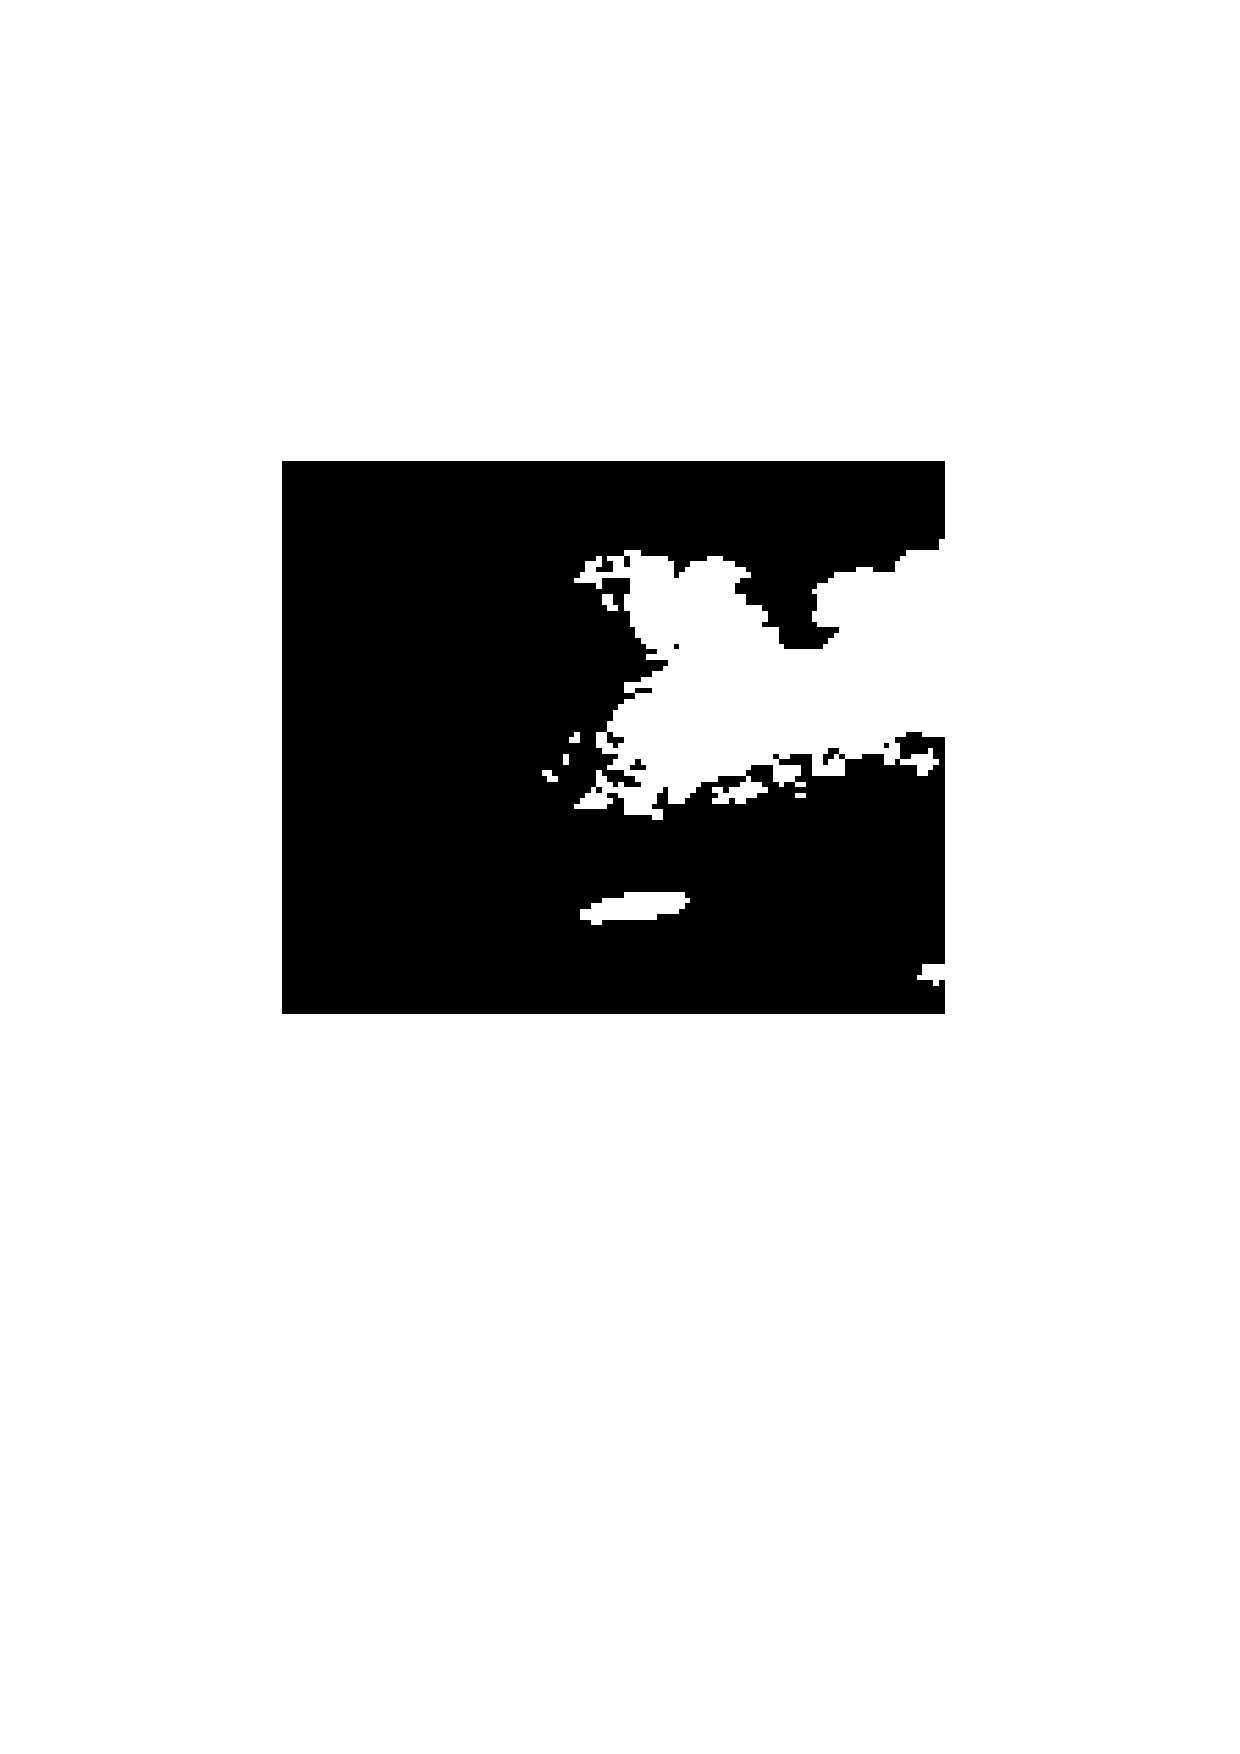
\includegraphics[height=0.25\textheight]{figures/binary}
	\caption{A binary map.}
	\label{fig:binary}
\end{figure}

\subsubsection{单阈值法}
首先介绍一种常用于工程实践中的地海杂波识别算法,单阈值法。通常,海洋和陆地杂波的差异在于,地杂波最大能量的频率几乎为零。 然而,海杂波存在沿着零频率对称的有两个类似的峰,称为布拉格峰。因此,我们可以使用频率$ f $来判别频谱数据的地海杂波属性。
\begin{equation}
f_{i, j}= \mathop{\arg\max}_{f} \ \ x(i, j, f)
\end{equation}
$x(i, j, f)$ 是在频率 $f_{i, j}$下的能量值。在已知 $f_{i, j}$ 的情况下, 我们需要和阈值 $\eta$ 比较来判断其地海属性。
\begin{equation}
	y_{i, j}= \left\{\begin{array}{ll}
		0&|f_{i, j}| > \eta, \\
		1&|f_{i, j}| < \eta
		\end{array}
		\right.
\end{equation}
0代表海洋,1代表陆地。
\subsection{我们的分类算法}
受电离层非平稳、时变等特性影响,天波超视距雷达杂波数据可能会出现较大波动。对这种波动不加处理会导致地海杂波识别结果不准确。在一个相对短时间内,电离层会保持一个较平稳的状态,也即同一距离、方位单元的地海属性不会发生变化。本章采用滑窗融合的方法对输入数据进行预处理。其基本思想是,将连续窗长时间内的相邻杂波数据进行加权融合得到新的频谱数据作为输入。

根据我们地海杂波频谱的实际数据及其反映的特点,构建了一个具有六层的基本卷积神经网络,如图\ref{fig:struct}所示,每层具有多个特征向量,每个特征向量具有多个神经元,\textcolor{red}{并且每个特征向量从提取输入的卷积滤波器的特征导出}。本章选择频谱向量中的连续范围作为池化区域(池化长度为2),并且只是池化相同的隐藏单元产生的特征。
\begin{figure*}[!t]
	\centering
	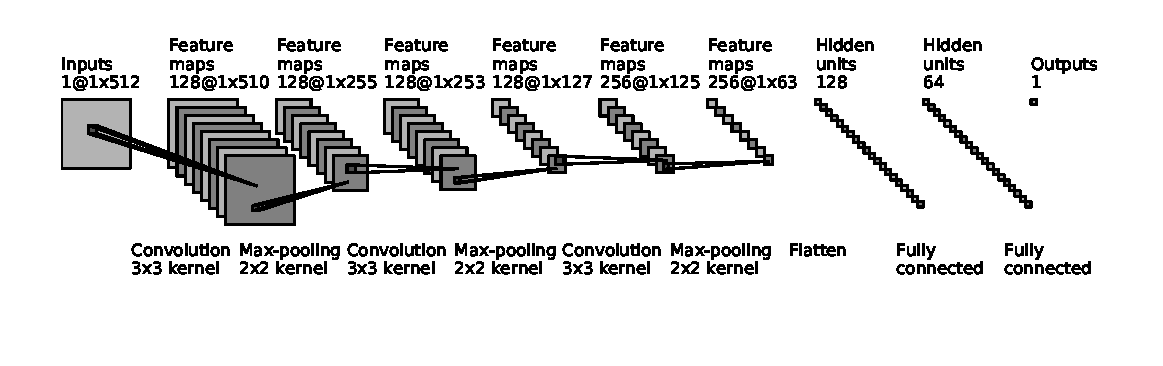
\includegraphics[width=\textwidth]{figures/struct}
	\caption{卷积神经网络结构}
	\label{fig:struct}
\end{figure*}

\subsubsection{池化层}
\textcolor{red}{由于我们雷达信号具有一种“静态性”属性,在一个数据区域有用的特征极有可能在另一个区域同样适用。因此,为了描述数据量较多的数据,一个很自然的想法就是对不同位置的特征进行聚合统计,例如,可以计算频谱数据上一段频率范围内的某个特征的最大值(或平均值)。这些经过采样的统计特征相比使用所有提取得到的特征不仅具有低得多的维度,同时还不容易过拟合,在一定程度上会改善结果。这种聚合的操作称为池化,常用的池化方法有平均池化和最大池化。由于这些池化单元具有平移不变性,所以即使频谱数据的布拉格峰经历了一个小的平移之后,依然会产生相同的池化的特征。
}

\textcolor{red}{这部分要结合实际问题讨论}

\subsubsection{训练算法}
传统的神经网络优化方法是mini-batch梯度下降。 这个想法是计算每次迭代的mini-batch梯度,然后更新参数。然而,这种方法有两个缺点,一个是学习率的选择是困难的,因为它对所有参数使用相同的学习率,故很难选择一个很合适的初值,另一个是趋向于收敛到局部最优。

在本章中,我们选择一种自适应算法Adaptive Moment Estimation,其具有自适应学习速率。该训练算法通过使用一阶矩估计和梯度的二阶矩估计来动态地调整每个参数的学习速率。每次调整后,每个迭代学习率都有明确的范围,使得参数更加稳定。

其基本的算法表示如下:

\textcolor{red}{写成算法图模式是否更好?}

\textcolor{red}{步骤1 : 输入地海杂波频谱序列,设其为1*N的序列,对其进行卷积运算,得到第一个卷积层,用C1表示。本章使用32个大小为1*3的卷积核,故特征向量中每个神经元与输入中的1*3的邻域相连,这样C1层中的特征大小就为1*(N-3)。又因为C1有128个可训练参数(每个滤波器具有3个单元参数和一个偏置参数,一共32个滤波器,共(1*3+1) *32 =128个参数),共128*(N-3)个连接,将连接通过ReLU激活层。
步骤2 : 对C1进行最大池化处理,该操作将相邻的多个特征采用一个特征进行代替。通过降低特征向量的长度,在减小了计算量的同时也在一定程度上修正了过拟合情形。
步骤3 : 将经过上述两个步骤获得的特征向量作为新的输入,重复多次步骤1至2(本章为三次),可以得到一个三阶段的卷积神经网络结构。上述多阶段卷积操作充分提取了输入向量的特征。
步骤4:构建输出层。拉平(flatten)步骤3获得的特征向量,以此作为卷积层到全连接层的一个过渡。在第一个全连接层的基础上添加dropout参数,然后添加第二层全连接,通过激活函数Sigmoid,获得分类结果的输出层。
步骤5:训练神经网络模型。在搭建好神经网络模型后,利用训练样本对该模型做进一步训练,其基本步骤如下:
步骤a、 初始化步长 ,矩估计的期望衰变率 ,初始参数 ,一阶矩与二阶矩变量 ,迭代次数 。
步骤b、从训练集中获取对应于目标 的具有 个样本的采样 ,其中 为批处理中一批样本的个数。
步骤c、计算梯度  ,其中 为对数损失函数,其定义为 。
步骤d、更新迭代次数 ,有偏一阶矩估计 ,有偏二阶矩估计 。
步骤e、修正一阶矩估计 ,二阶矩估计 。
步骤f、更新参数  ,其中 用来保持稳定性,同时判断是否满足结束条件,如果不满足重复步骤b-f。
步骤6:在线识别。将需要识别的样本进行融合预处理,其基本思路为维护一个滑窗,对于某滑窗内的对应分辨单元的数据进行加权融合,其权值与窗长需要根据实验数据进行确定(本章窗长选择为5),然后将融合后的数据通过步骤5获得的训练好的模型,得到最终识别结果。}

\subsection{增量学习}
随着时间的迁移,天波超视距雷达的观测范围或者是运行参数可能会发生大的变化,使得目前的训练结果无法很好的满足新的需求,于是本文设计了一种基于增量学习的训练方法。对于新的频谱数据集一般会相比于原数据集更小,所以重新训练常常无法取得一个很好的结果,对原始训练结果进行微调是十分必须的。一般来说,DCNN的比较靠前的层所包含的特征更一般化,而更靠后的层会越来越特定于该频谱数据中包含的分类细节。所以一个比较好的方案是保持前面的一些层固定,只微调网络后面的一些层。另一方面,由于原始数据训练出的DCNN的权重是相对较好的,故需要给正在被微调的DCNN权重使用较小的学习率和学习衰减率。
\section{地海杂波分类评估}
在本节中,我们利用实际数据对我们提出的算法的性能进行评估。
\subsection{数据集分析}
我们所有的数据都来自不同时间,不同地点和不同雷达配置的频谱数据。我们分析了所有频谱数据,并选择一些\textcolor{red}{典型}的频谱数据,如图\ref{fig:spectrum}所示。
\begin{figure}[!t]
	\centering
	\subfloat[地杂波频谱]{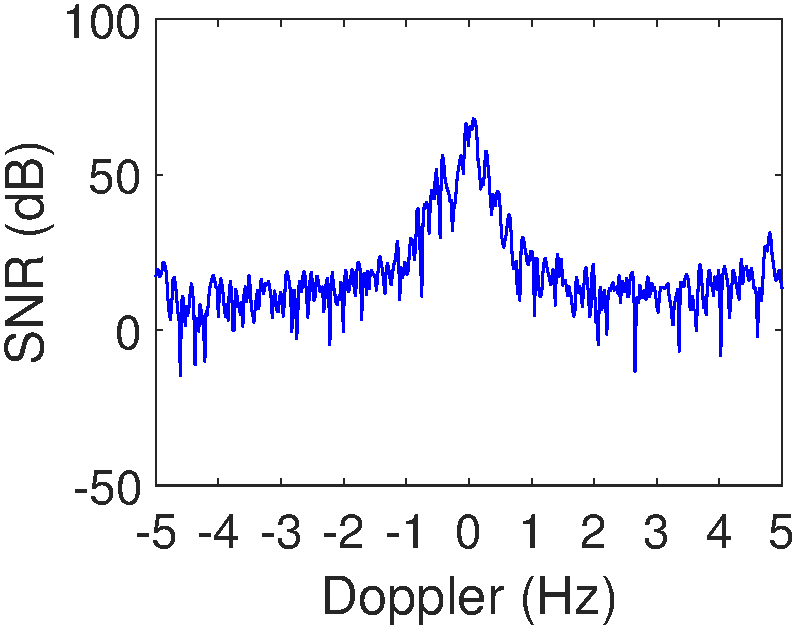
\includegraphics[width=0.4\textwidth]{figures/land}%
		\label{fig:land}}
	\hfil
	\subfloat[海杂波频谱]{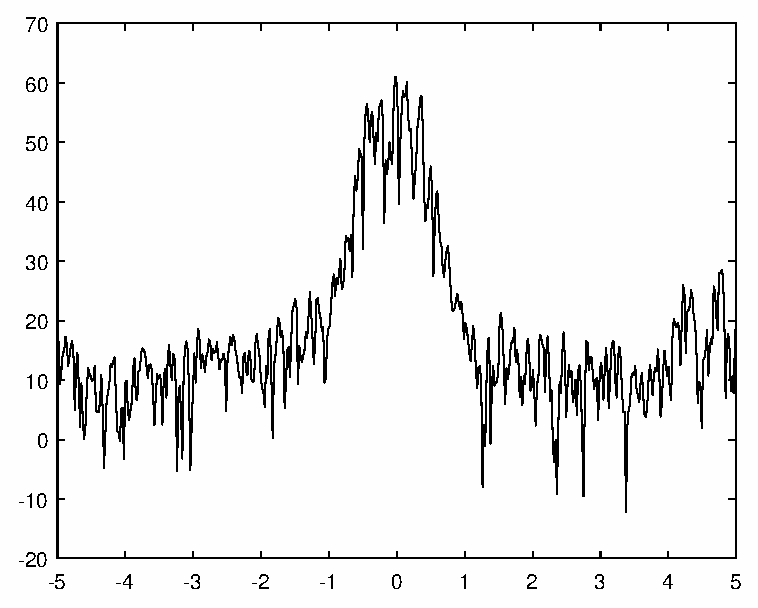
\includegraphics[width=0.4\textwidth]{figures/sea}%
		\label{fig:sea}}
	\caption{两幅无法轻易区分的地海杂的频谱波示意图。 图 \ref{fig:land} 的布拉格峰具有小的频偏,图 \ref{fig:sea} 作为海杂波却无法容易的分辨出布拉格峰.}
	\label{fig:spectrum}
\end{figure}

\subsubsection{数据集分组}
\textcolor{red}{按照文章重新修改}

在本章的问题中,当雷达配置发生变化时,我们会获得不同的频率范围和精度频谱数据。例如,一些频谱数据的频率变化范围为-5Hz到5Hz、具有512个相干积累点,而另一些数据的频率变化范围为-10Hz到10Hz、相干积累点数为256个。因此,基于这两个条件,我们将所有数据分为4组:
\begin{itemize}
	\item 组 A: 如图\ref{fig:case128}所示,具有128个相干积累点数,频率变化范围为-5Hz到5Hz;
	\item 组 B: 如图\ref{fig:case256}所示,具有256个相干积累点数,频率变化范围为-5Hz到5Hz;
	\item 组 C: 如图\ref{fig:case512}所示,具有512个相干积累点数,频率变化范围为-5Hz到5Hz;
	\item 组 D: 如图\ref{fig:case1024}所示,具有1024个相干积累点数,频率变化范围为-5Hz到5Hz;
\end{itemize}
我们只选择了上述四个具有典型意义的分组的数据来进行验证,舍弃了其余类型的与他们相似的数据,例如频率变化范围为-10Hz到10Hz的具有512个相干积累点的数据,这与组B的数据基本相同。
\begin{figure*}[!t]
	\centering
	\subfloat[组 A]{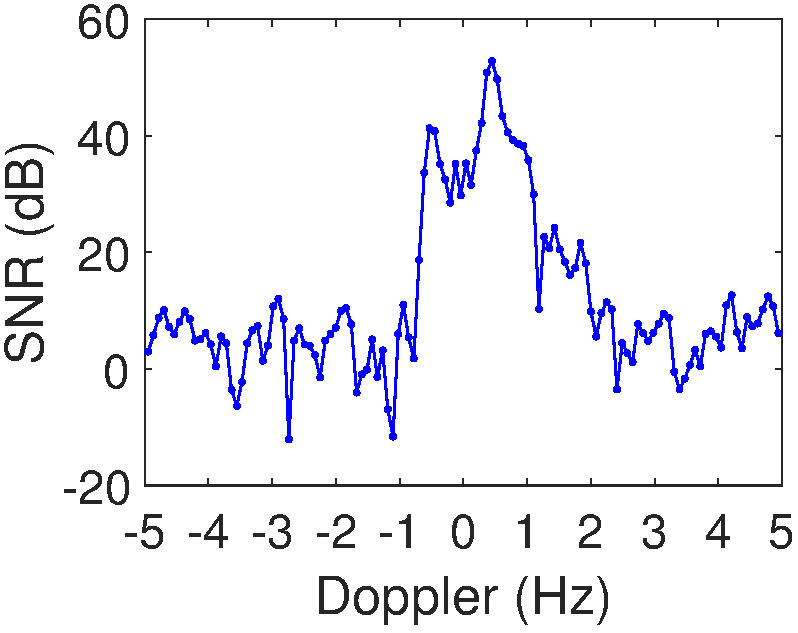
\includegraphics[width=0.4\textwidth]{figures/group128}%
		\label{fig:case128}}
	\hfil
	\subfloat[组 B]{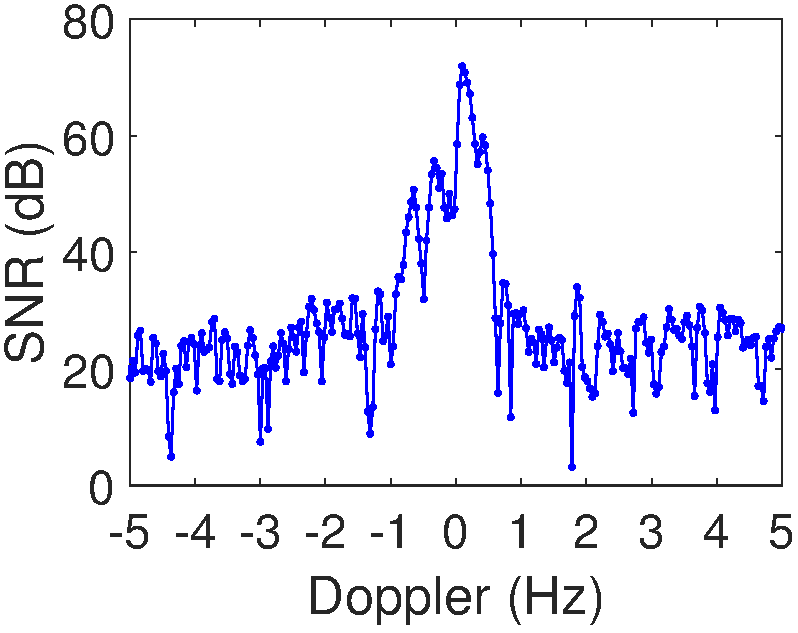
\includegraphics[width=0.4\textwidth]{figures/group256}%
		\label{fig:case256}}
	\centering
	\subfloat[组 C]{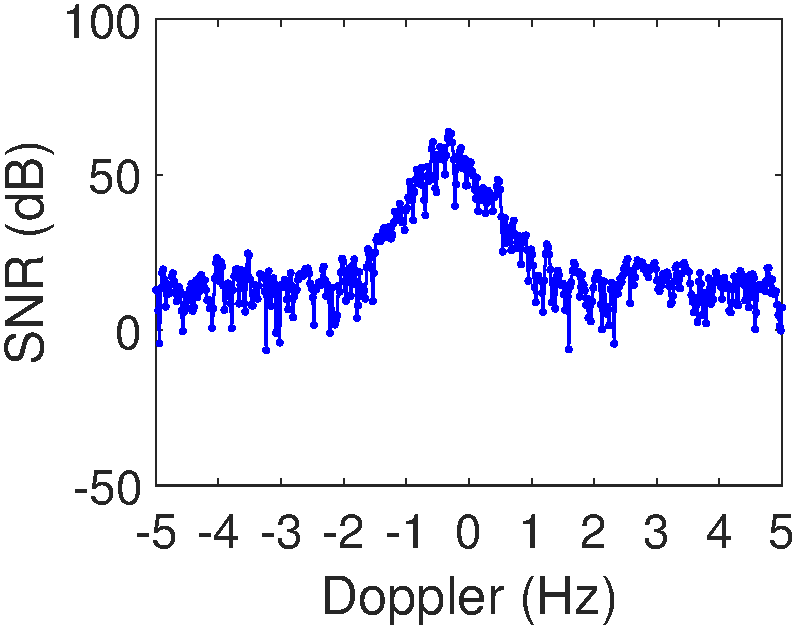
\includegraphics[width=0.4\textwidth]{figures/group512}%
		\label{fig:case512}}
	\hfil
	\subfloat[组 D]{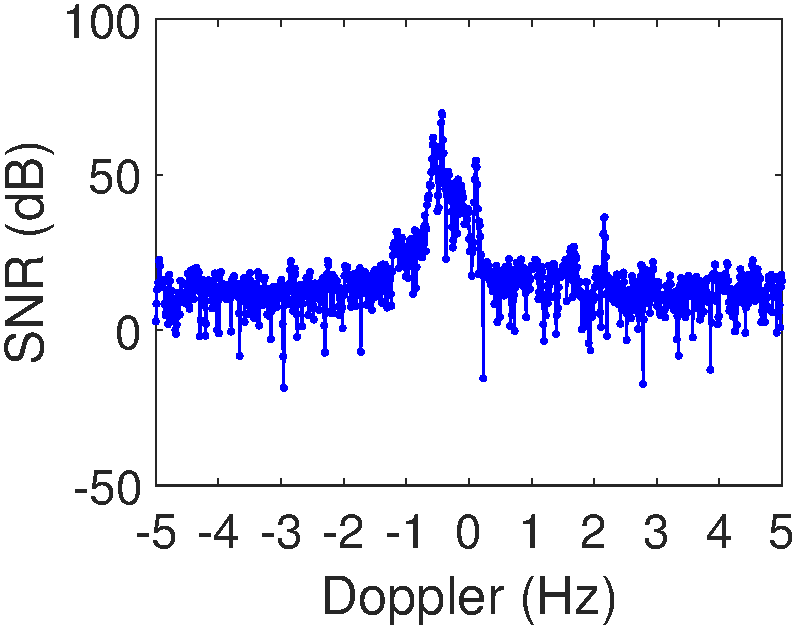
\includegraphics[width=0.4\textwidth]{figures/group1024}%
		\label{fig:case1024}}
	\caption{不同组数据的频谱对比示意图}
	\label{fig:group}
\end{figure*}
\subsection{算法实现}
\textcolor{red}{对其余两个算法的介绍}
我们将我们的算法与传统的单特征识别算法和SVM算法进行对比。选择SVM的地海杂波的三个特征是:
\begin{itemize}
	\item 最大后向散射幅值
	\item 频谱中最大与次大幅值频率之差
	\item 频谱中最大与次大幅值幅度之差
\end{itemize}
为了确保我们有足够的数据来训练和测试我们的算法,我们选取了不同的雷达工作条件、天气、时间的多组数据(每组约有20000个频谱数据)。我们随机选择其中$70\%$的数据作为训练数据,$20\%$作为交叉验证数据,其他数据用作测试数据。

\textcolor{red}{测评计算公式叙述}

\subsection{仿真验证}
为了验证我们的深度卷积网络的泛化能力,我们利用了四组数据测试了我们的方法,其不同组数据的损失函数如图\ref{fig:group_results}所示,结果表明我们的算法可以在不同的数据集组中获得良好的结果。虽然,对于相同的神经网络结构,第一个数据集需要最多的迭代次数才能收敛,这是因为当频率和相干累计点的比例变小时信息或者说特征也随之减少,故需要较多的迭代次数。
\begin{figure}[!t]
	\centering
	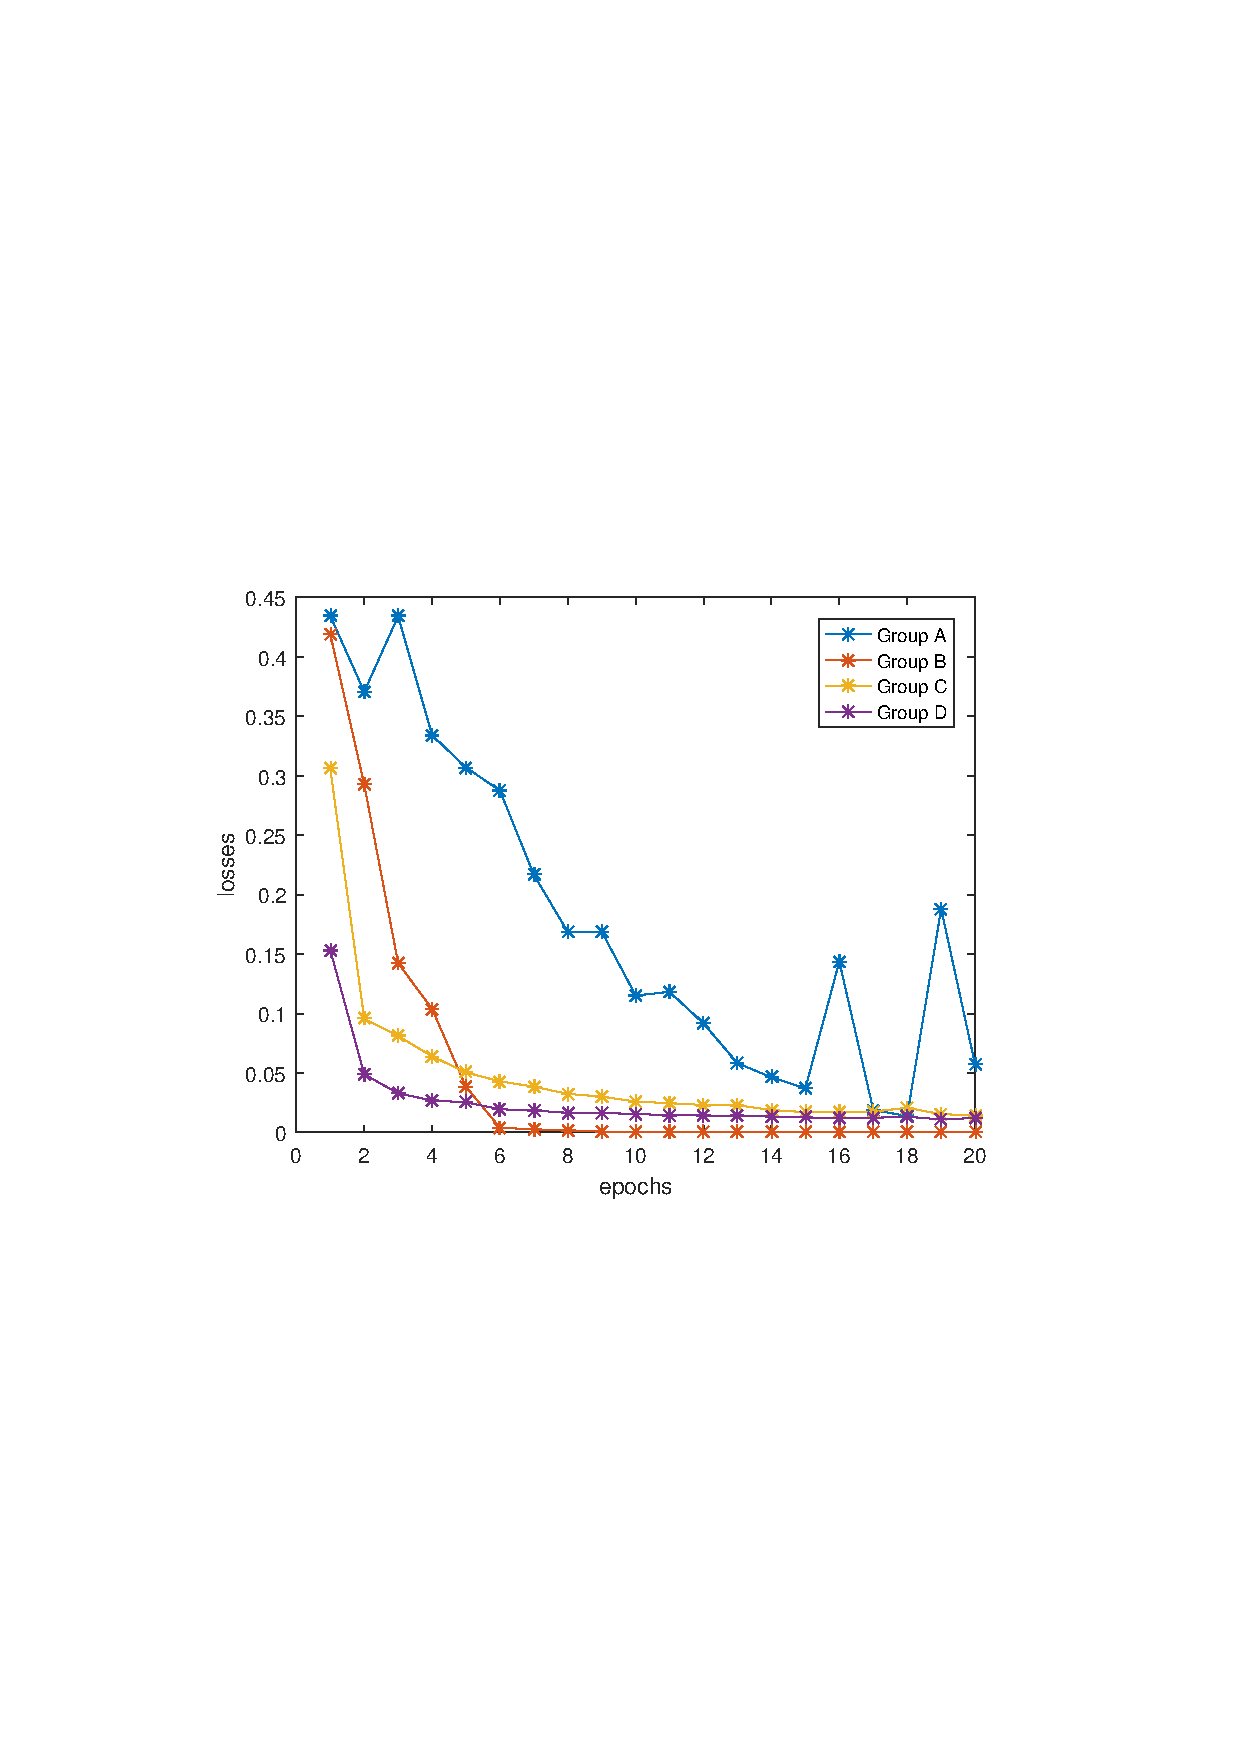
\includegraphics[width=\textwidth]{figures/group_results}
	\caption{不同数据集损失函数对比图。}
	\label{fig:group_results}
\end{figure}
正如上面描述的,还有另外两种常用的算法来做地海杂波的识别。我们利用实际数据进行实验来对三种算法进行了对比。实验结果如表\ref{tab:methods}所示,可以明显的看到,我们的算法在识别正确率和匹配准确率均为最优。并且,我们可以发现SVM和基准方法都匹配到了错误的区域。\textcolor{red}{此外,当通过整个世界地图找到最大的匹配率时,三种方法与其配对地图在一段时间内的交配率似乎有所不同。}

\textcolor{red}{添加对于三个判断结果参数的设计}
\begin{table}[!t]
	\renewcommand{\arraystretch}{1.3}
	\caption{三种算法识别正确率与匹配正确率计算.}
	\label{tab:methods}
	\centering
	\begin{tabular}{c|ccc}
		\hline
		& 我们的算法 & 支持向量机 & 单阈值算法 \\
		\hline
		识别正确率 & 99.69\% & 92.44\% & 81.85\% \\
		\hline
		最大匹配正确率 & 88.99\% & 22.77\% & 23.48\% \\
		\hline
		匹配正确率 & 88.99\% & 81.31\% & 88.21\% \\
		\hline
	\end{tabular}
\end{table}

图\ref{fig:sizes}展示的是在样本集大小不同的情况下,我们的算法与基准算法的平均分类准确率的对比图。由于基准方法仅使用根据先验知识得到的阈值,因此随数据集增长其识别准确度变化不大,而我们的深度卷积神经网络的算法随着数据集内样本数量的增加,准确度有着显著提升。
\begin{figure}[!t]
	\centering
	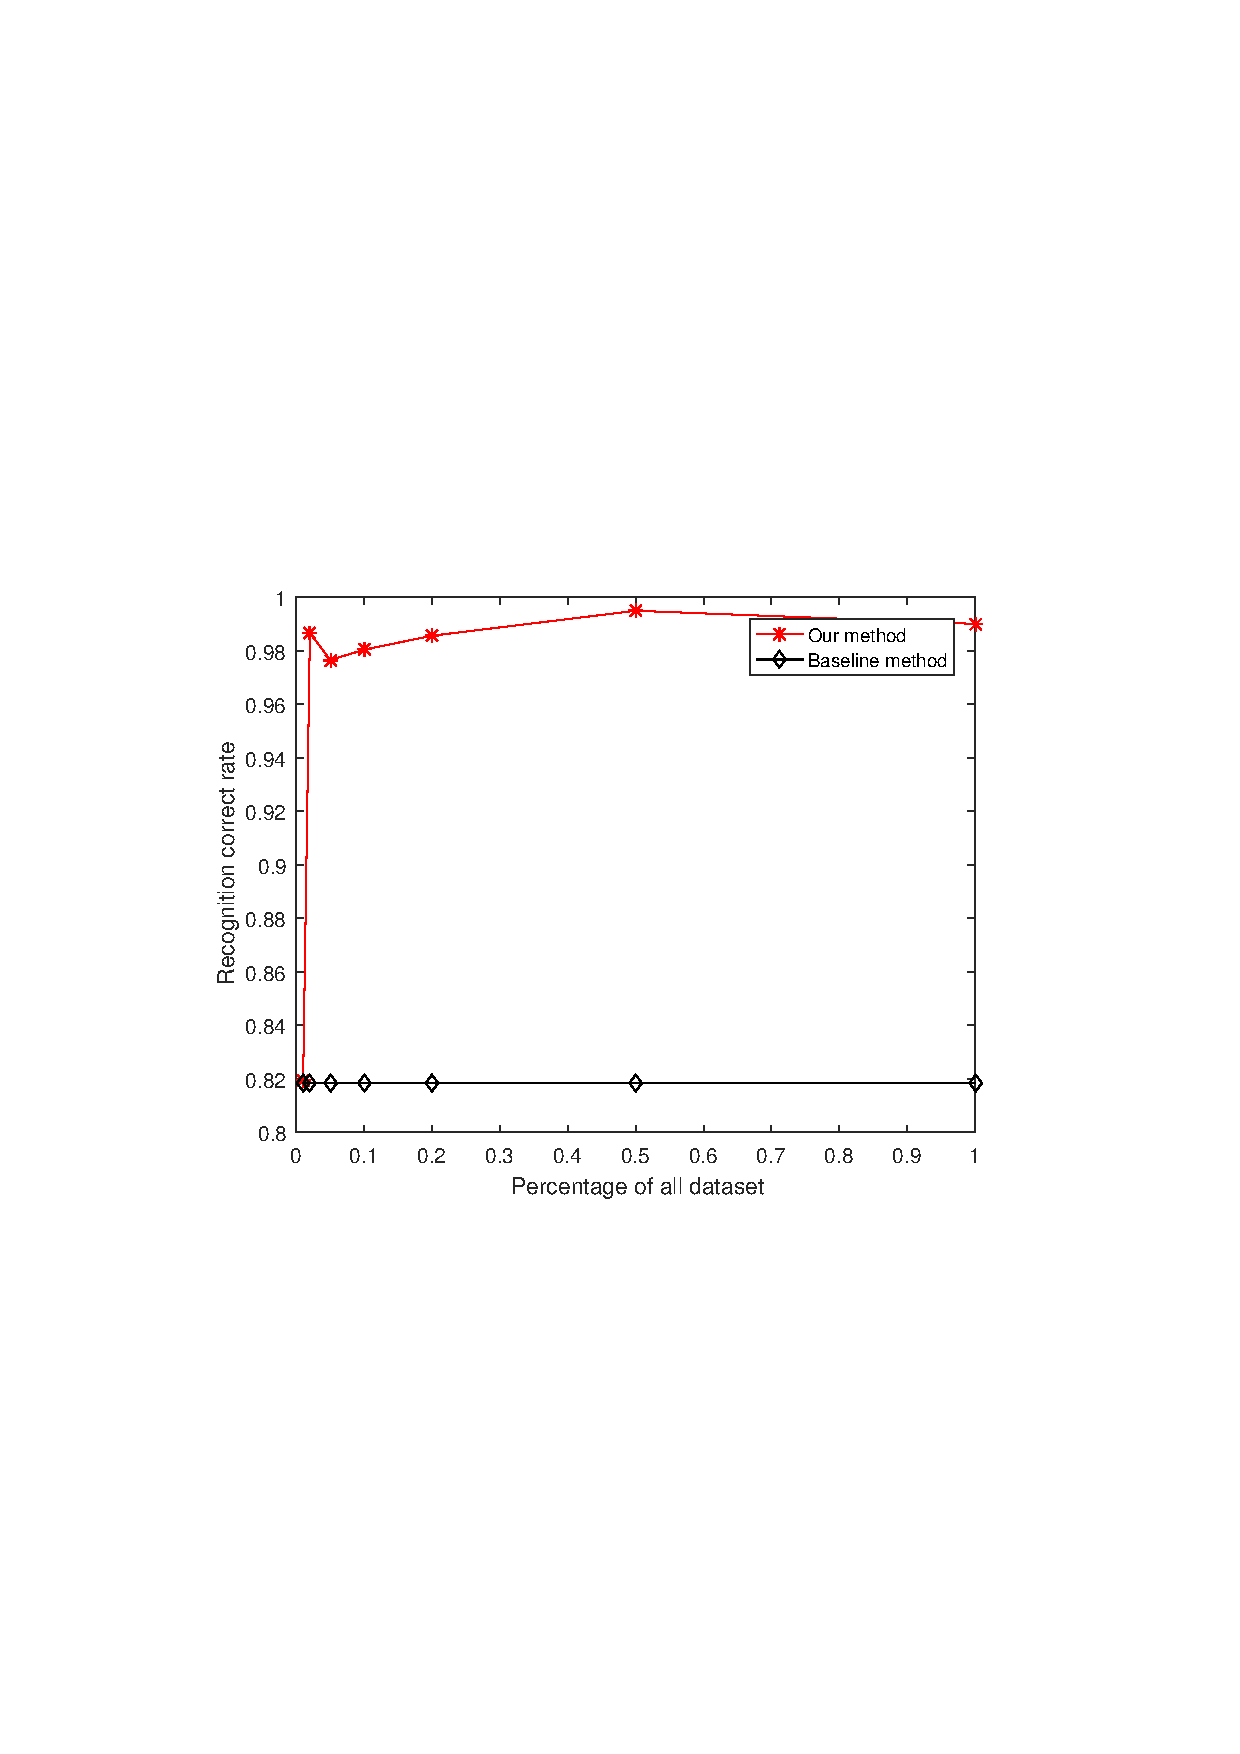
\includegraphics[width=\textwidth]{figures/sizes}
	\caption{不同数量数据集的分类准确度对比曲线图}
	\label{fig:sizes}
\end{figure}

众所周知,卷积神经网络的参数对于最终分类识别的准确率起着重要的作用。因此,我们需要对参数的选择进行一些分析。首先,我们分析在批大小(Batch Size)和迭代次数变化时,验证集数据的分类准确度。如图\ref{fig:epoch}所示,我们可以发现识别准确度随着迭代次数的增加而增长。而当批长度变大时,收敛速度加快。
\begin{figure}[!t]
	\centering
	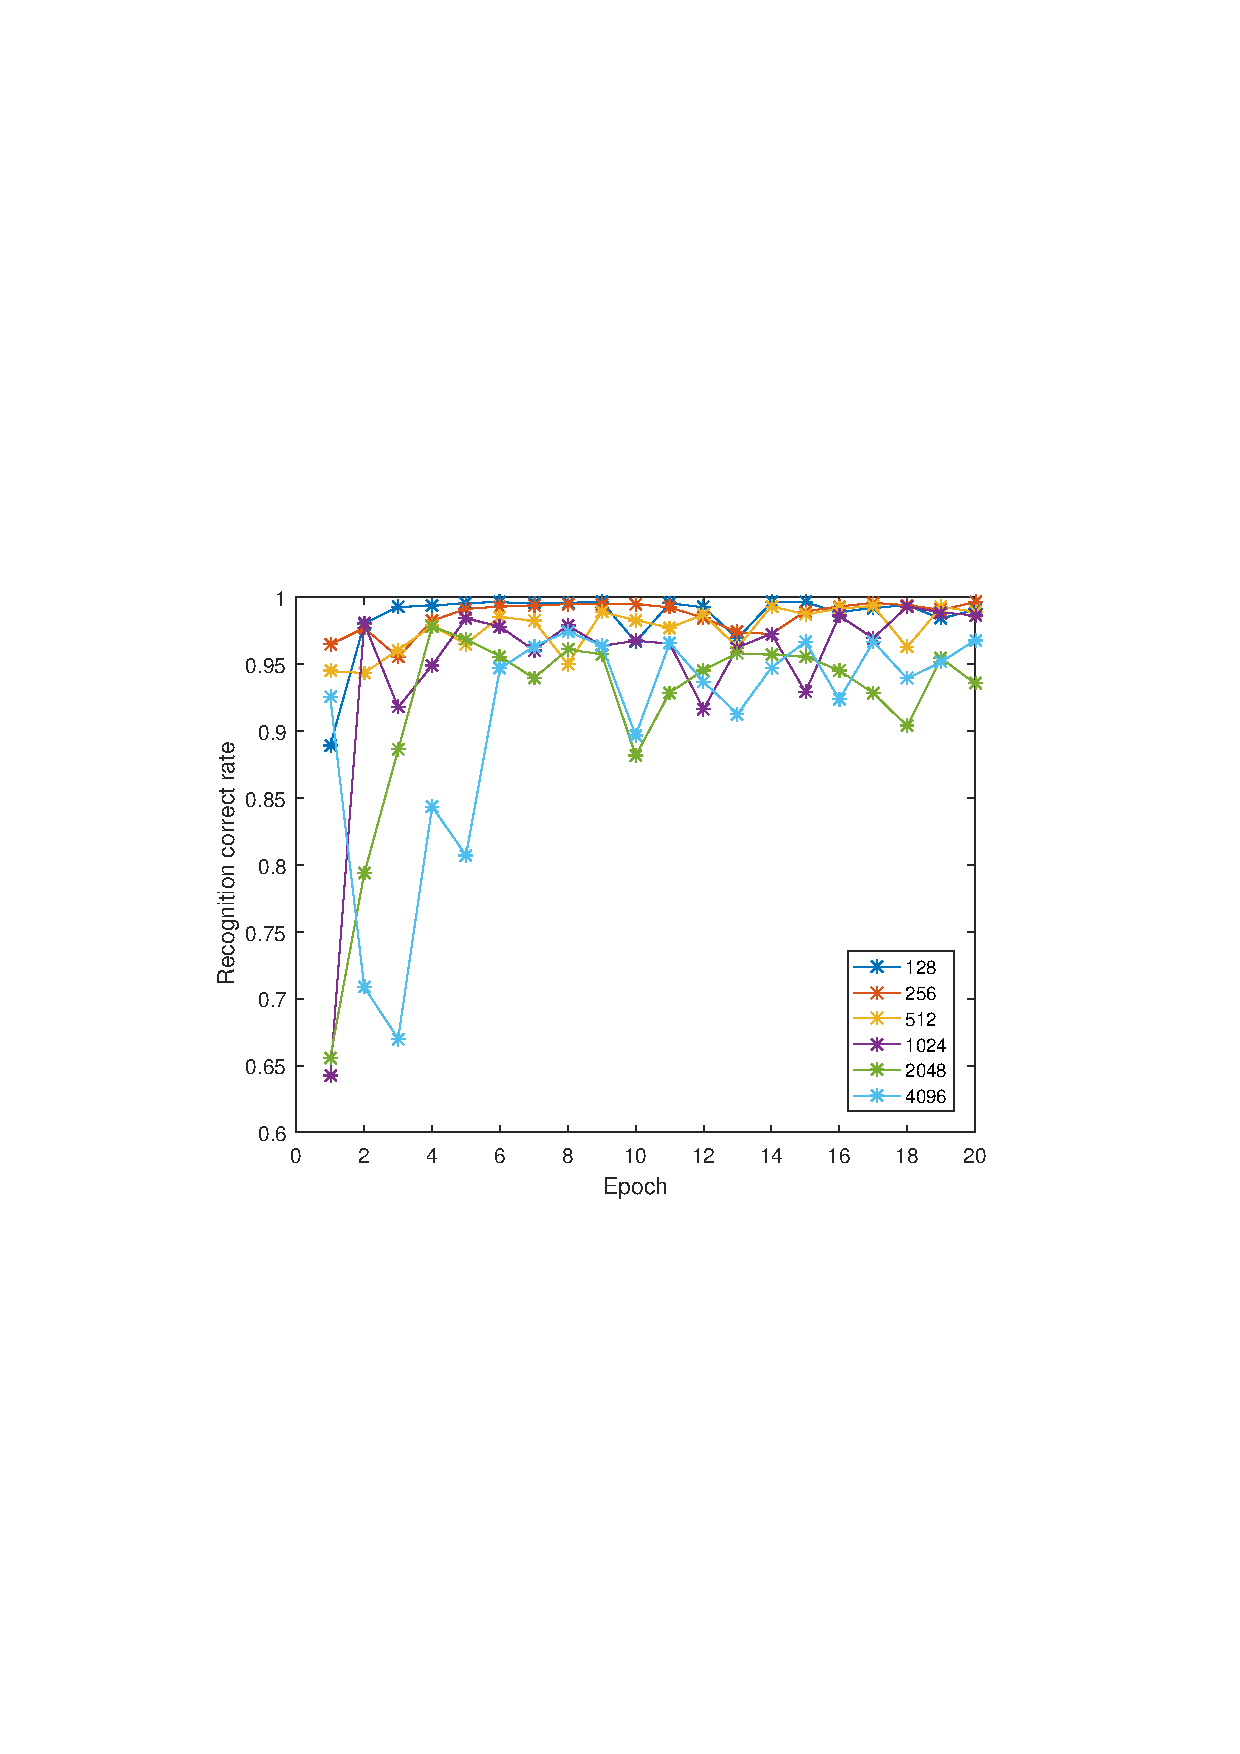
\includegraphics[width=\textwidth]{figures/epoch}
	\caption{不同批长度下,分类准确度与迭代次数曲线图}
	\label{fig:epoch}
\end{figure}

融合预处理参数设计由于滑窗算法的很重要的一个参数就是窗长,针对于本问题主要考虑到电离层会发生变化,过长的窗长对无法及时的响应电离层的变化,影响识别准确率以及地图匹配精度。为了取得一个合适的窗长,我们首先利用不同窗长平均融合后的数据进行测试,得到图 20的结果,该结果也证明了在窗长过长时候,准确率会下降的结论,当窗长过大时准确率会降到比窗长为1时还要低。 图 23 不同窗长识别结果对比图为了进一步比较权重的变化对于识别结果的影响,我们设窗长为 ,样本 的权重为 ,则有融合后的样本为 ,当取权重为 时,得到下面结果,故根据实验结果,本课题最终选择窗长长度为3 图 24 更改权重后不同窗长识别结果对比4.2目标定位精度修正验证由于缺乏实际的 变换相关的航迹信息,故无法对定位精度修正系数进行一个很好的验证。这里我们采用地图变换的过程来进行辅助验证。其基本流程与目标的定位精度修正类似。首先将整个匹配地图划分为很多小的匹配区域,然后对于每个匹配区域分别进行修正系数计算。

如前面所描述的,我们利用融合的方法来减少由于某一帧数据中某距离方位单元由于出现的随机噪声对于我们识别结果的影响。图\ref{fig:window}显示匹配率随着窗口长度的增加首先提高,然后减小。这是因为当窗口过长时,由于天波雷达的采样周期较长,这个期间内,雷达的频谱可能已经出现了一定程度的变化,这回影响最终的识别结果。
\begin{figure}[!t]
	\centering
	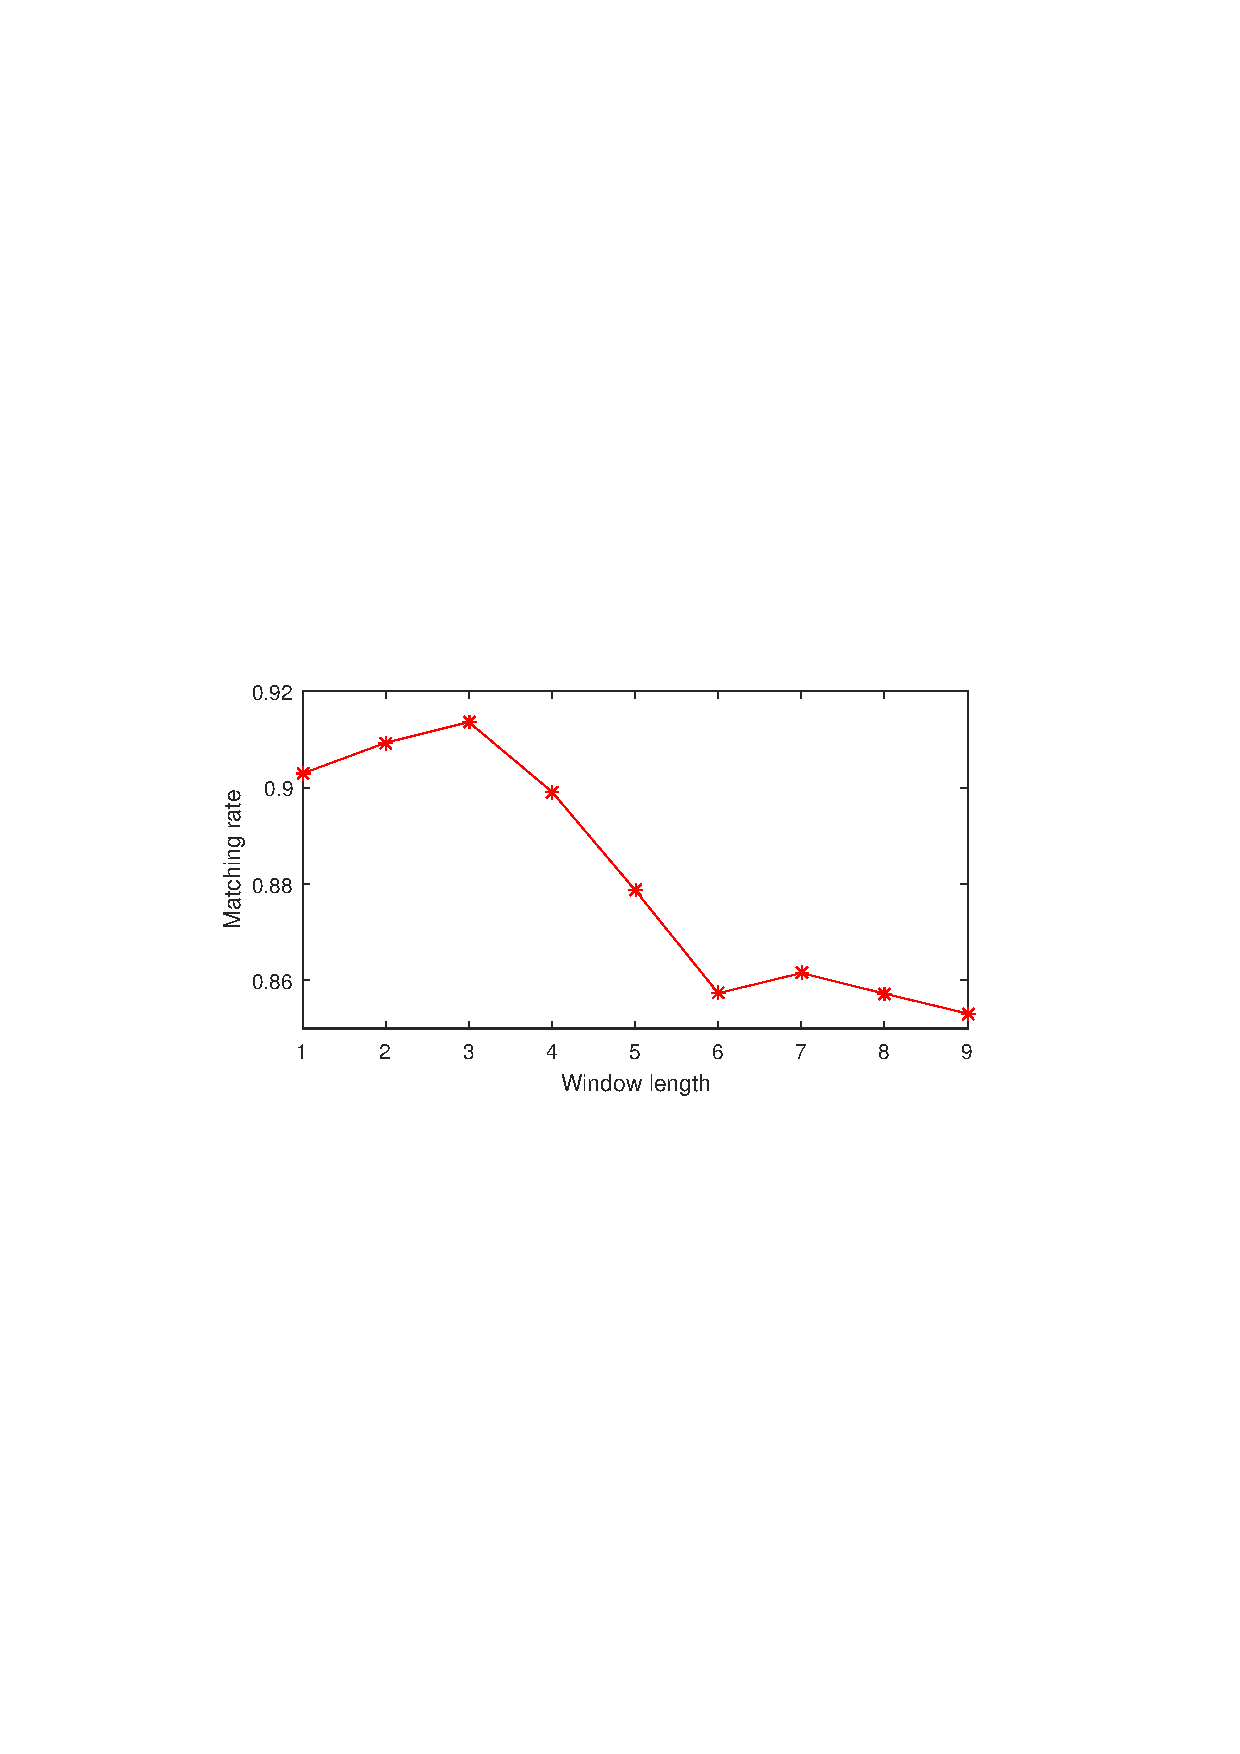
\includegraphics[width=\textwidth]{figures/window}
	\caption{The matching rate against fusion window length.}
	\label{fig:window}
\end{figure}
为了找出区分识别结果中海洋与陆地的最佳阈值,我们使用不同的概率阈值计算相同测试数据的正确率。图\ref{fig:threshold}显示,\textcolor{red}{随着阈值越大,增长速度越慢,速率越快}。另一方面,当阈值仅为$0.01$时,识别率仍高于$0.86$。这说明我们的方法的分类结果的概率值均处于较高的水平,如\ref{fig:prob}所示。
\begin{figure}[!t]
	\centering
	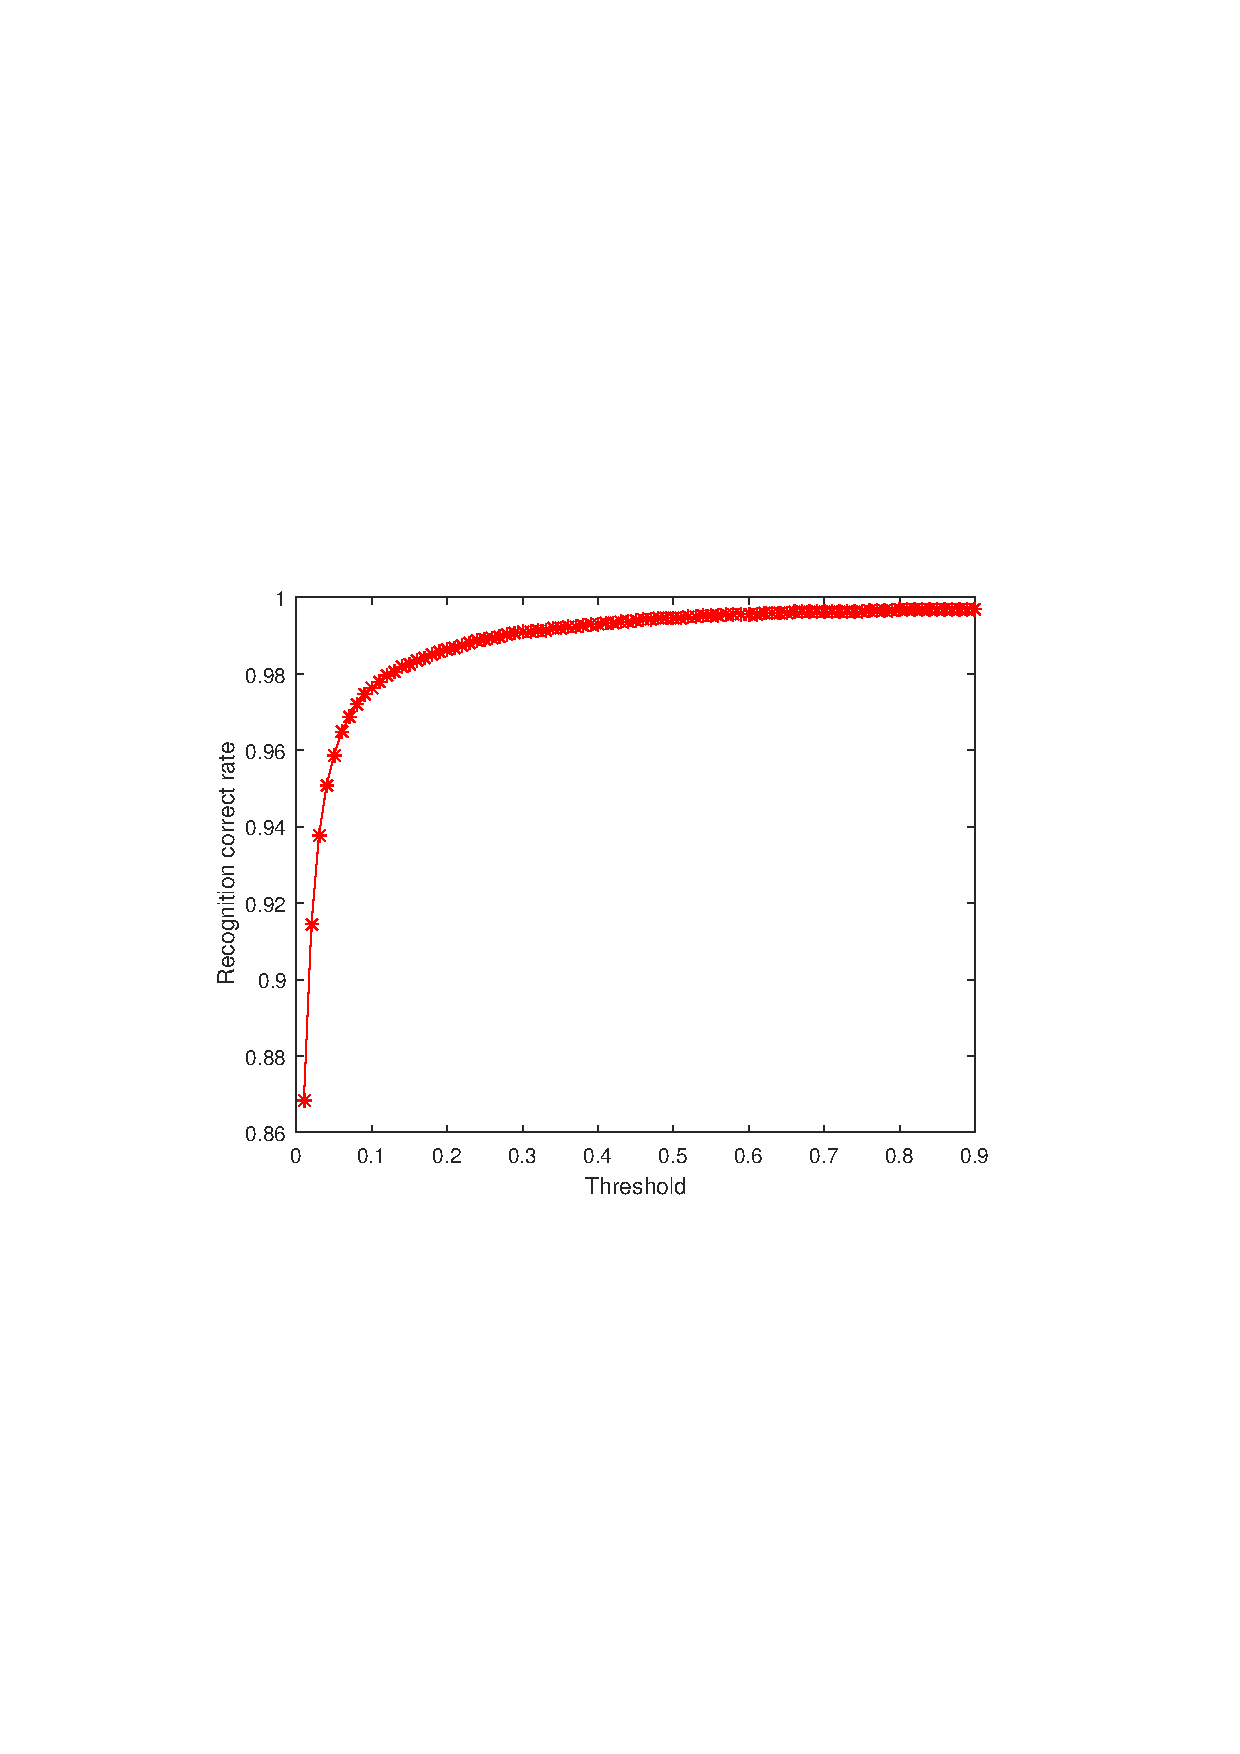
\includegraphics[width=\textwidth]{figures/threashold}
	\caption{识别率与概率阈值曲线图.}
	\label{fig:threshold}
\end{figure}
\begin{figure}[!t]
	\centering
	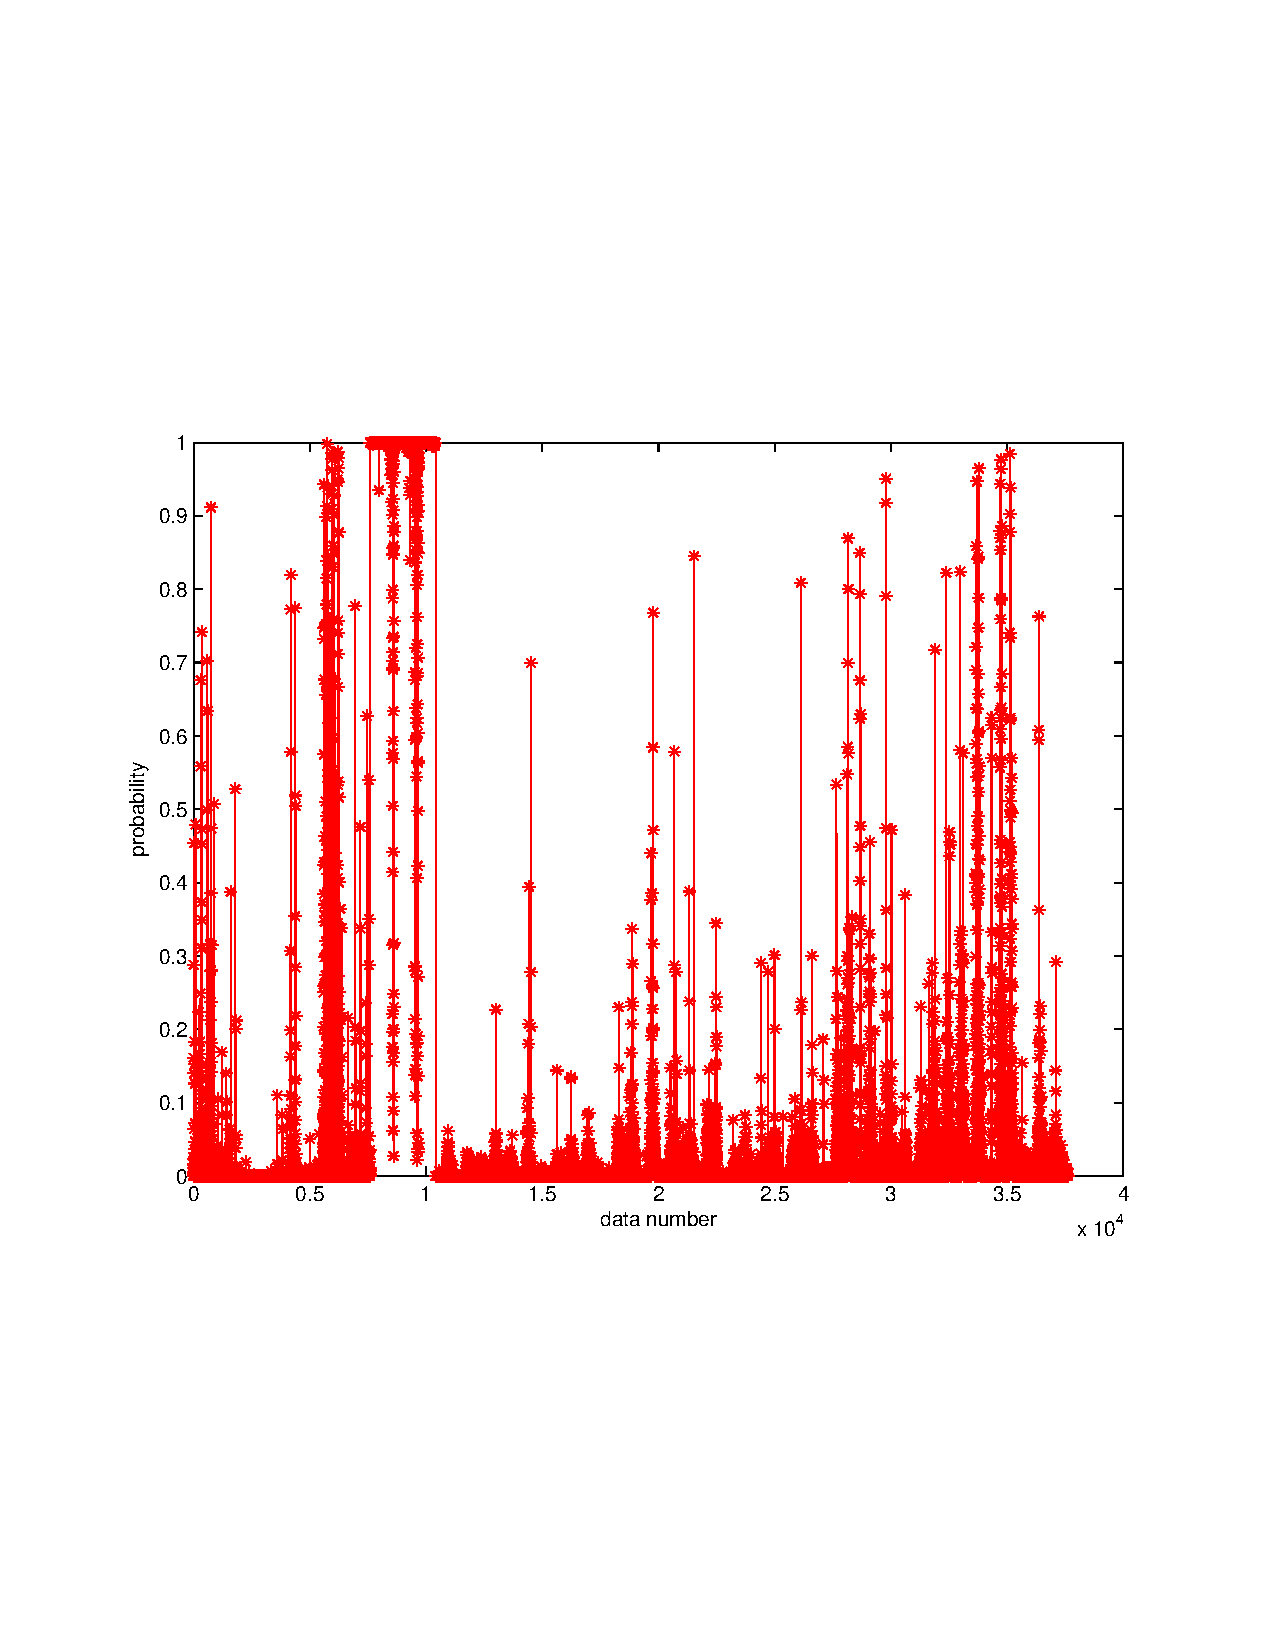
\includegraphics[width=\textwidth]{figures/prob}
	\caption{不同帧数据识别结果概率值}
	\label{fig:prob}
\end{figure}
%\begin{itemize}
%	\item different window and no window
%	\item figures of loss function with time
%	\item dropout changes
%	\item probability threshold changes
%
%	\item fusion and not fusion
%\end{itemize}
\subsection{特征可视化}
\textcolor{red}{该部分需要添加详细的内容}

识别结果的理论分析上面利用大量的测试数据的识别结果以及地图匹配结果对于算法进行了验证,这里我们通过理论分析,验证了算法的合理性。通过计算当输入数据的某个数据点发生变化时输出梯度的变化,得到每一个数据点对于输出梯度的影响,从而得到该频谱数据关注度图。图\ref{fig:visfeature}中红色圆圈部分表示主要利用的特征所在多普勒频率,可以很直观地看出,对于下图这样的海杂波布拉格峰附近频点的数据被关注比较多,另一方面同时兼顾了其余频点的特征,提高了识别准确率。 

卷积神经网络方法有一个问题是其为一个黑盒操作,我们无法直观地看到其用于分类的特征。因此,为了在理论上对于我们算法的有效性进行分析。在本节中,我们使用基于梯度变化的可视化方法,其思想为利用我们已经训练好的模型展示对于其最终判断测试结果为正或者为负主要利用的频谱特征点。我们定义频谱数据序列为$ S = \{s_1, s_2, .., s_n\} $,其中$n$是频谱序列中的点数,设输出概率为$p(S)$。那么,我们可以得到式\ref{equ:ps}:
\begin{equation}
p(S) = w^TS+b,
\label{equ:ps}
\end{equation}
其中$ w $和$ b $分别是我们的模型的权重和偏差。实际上,这里的权重$ w $表示对应点的重要性。在我们的模型中,类概率函数$p(S)$是高度非线性函数,这里使用泰勒方法近似$p(S)$。为了简化计算,我们使用一阶泰勒展开:
\begin{equation}
w = \frac{\partial{p}}{\partial{S}}{\mid}_{s_i}
\label{equ:w}
\end{equation}

\textcolor{red}{因此,我们以通过反向传播计算得到$ w $的方程式\ref{equ:w}(todo:详细描述)。图\ref{fig:vis}显示,特征点主要集中在我们预期的数据上。}
\begin{figure}[!t]
	\centering
	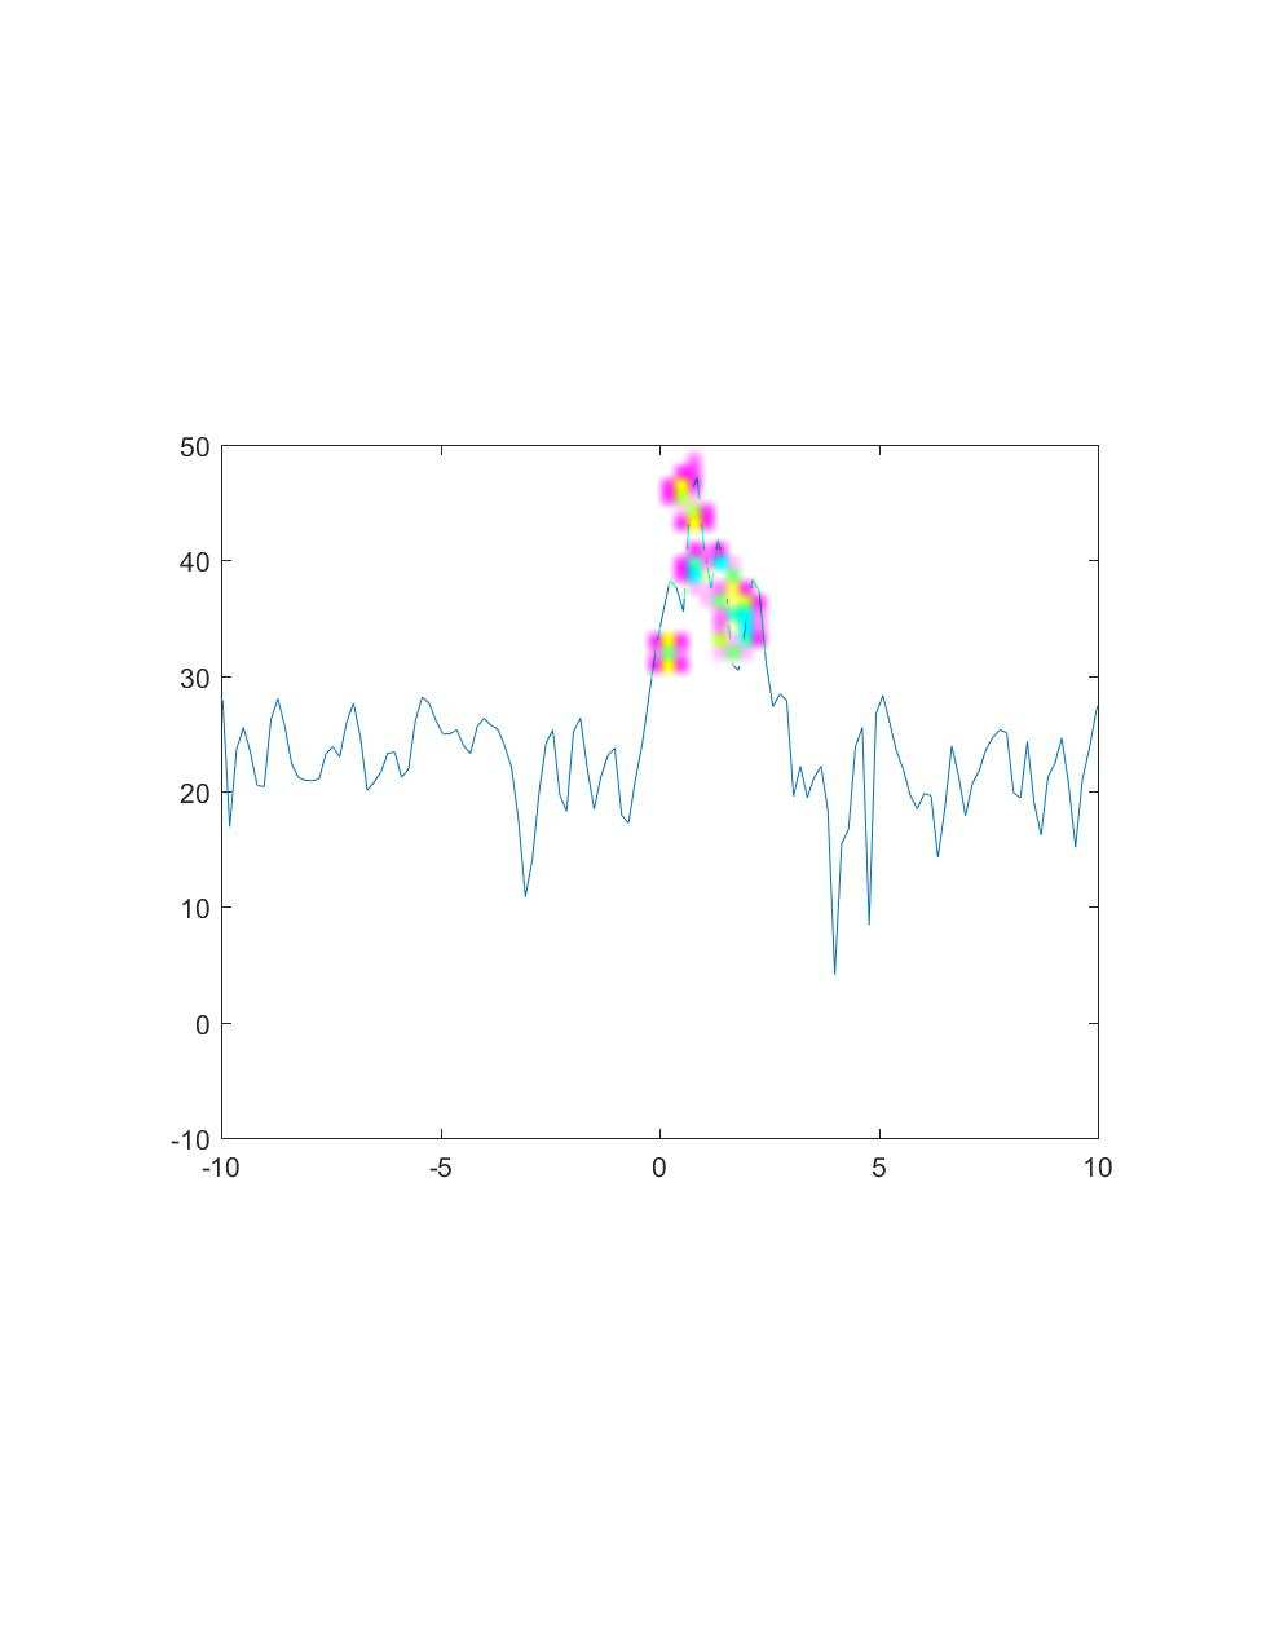
\includegraphics[width=\textwidth]{figures/heatmap.pdf}
	\caption{特征重要程度热力图。}
	\label{fig:vis}
\end{figure}
\begin{figure}[!t]
	\centering
	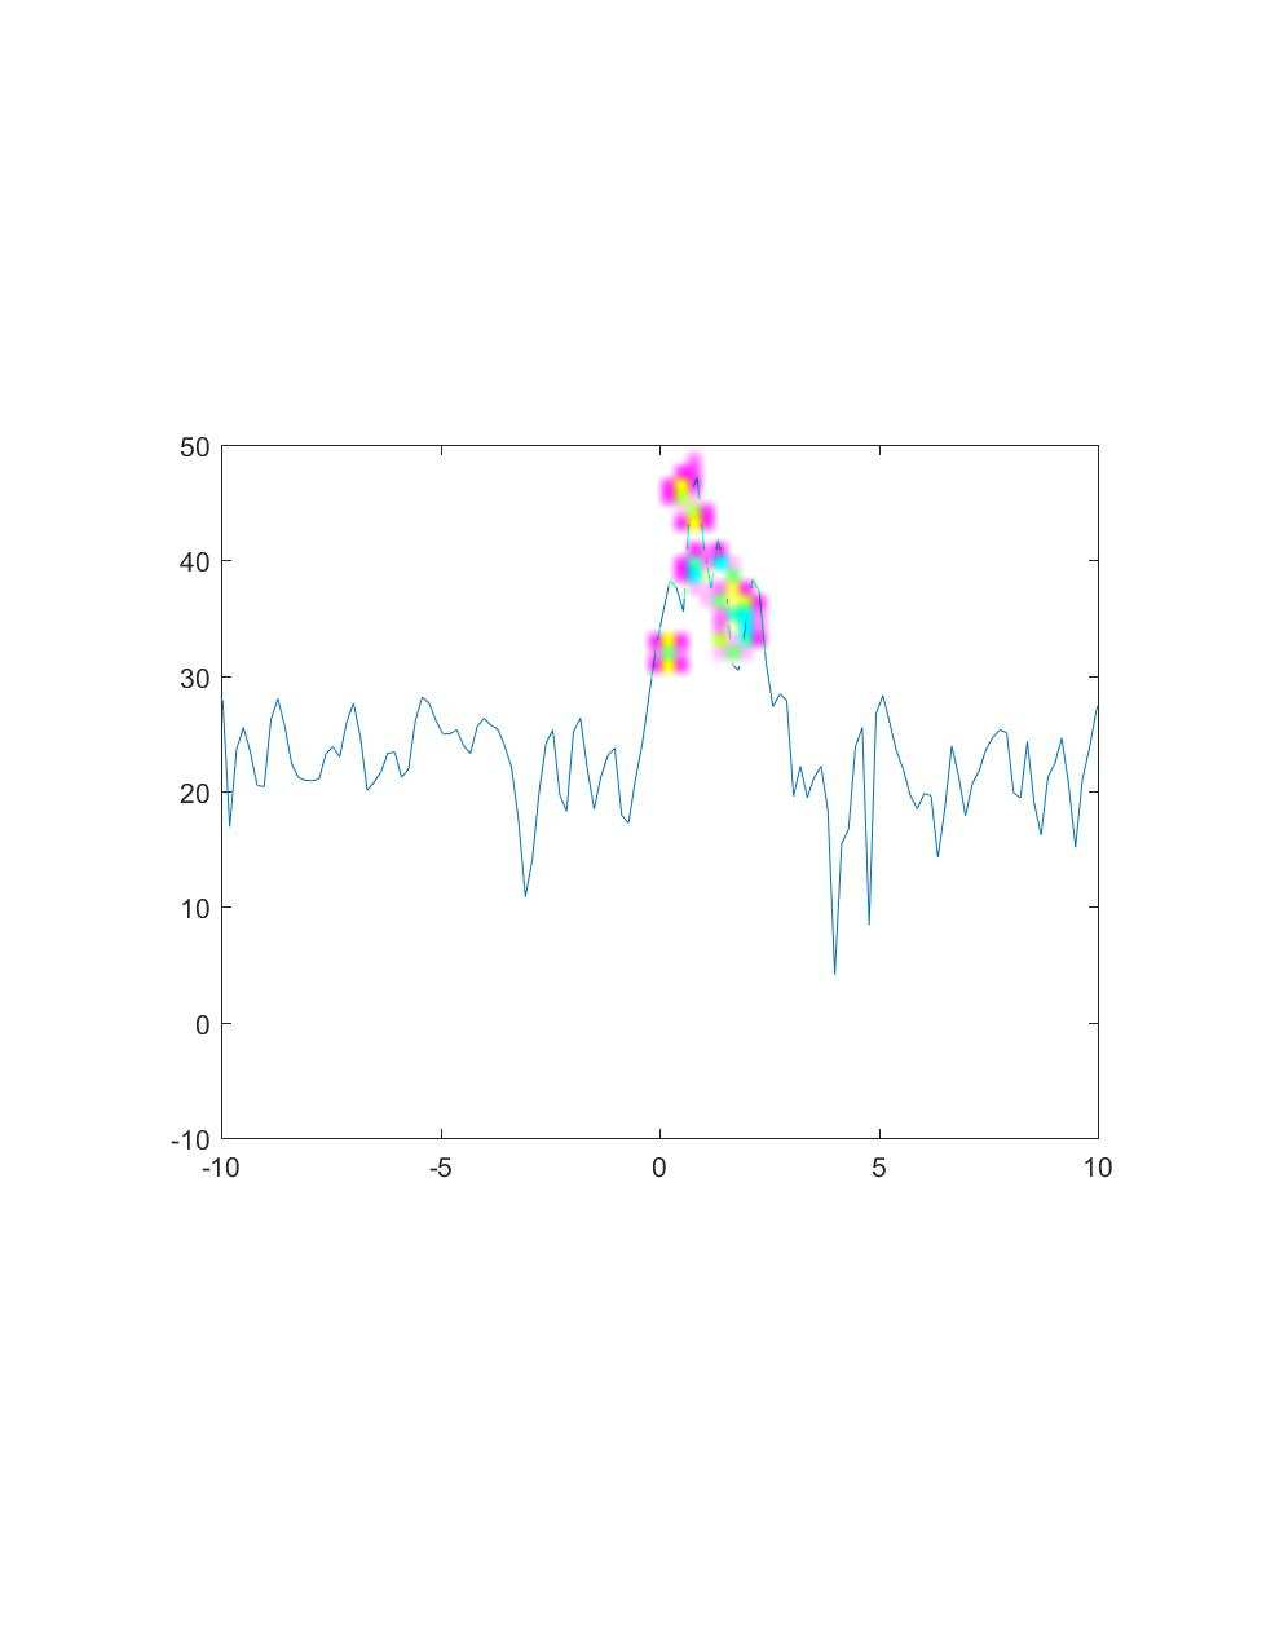
\includegraphics[width=\textwidth]{figures/heatmap.pdf}
	\caption{某距离方位单元海杂波频谱数据关注度图
	。}
	\label{fig:visfeature}
\end{figure}
\section{小结}
在本章中,我们提出了基于卷积神经网络天波雷达地海杂波识别的新算法。其主要克服了传统的阈值识别方法或支持向量机算法根据经验从频谱数据中提取特征,导致操作复杂度高,分类精度低的缺点。同时,我们将我们的算法与传统算法和支持向量机算法进行了对比。实验结果表明,我们的方法在地海杂波识别问题上更加有效以及抗干扰性能更强。在更高精度的识别结果的帮助下,我们可以得到更加精确的修正系数,可以为目标检测和跟踪问题提供非常大的帮助。